
\documentclass[10 pt]{book}

%  Standard packages
\usepackage{graphics,epstopdf,overcite,amsmath, color}
%\usepackage{rotating}

\usepackage{colortbl}  % For colors in tables

%  for making index, using landscape mode, for multi page tables, supertabular??
\usepackage{makeidx, lscape, longtable, supertabular}
\usepackage{tocloft}

%  Used for drawing lines in figures
\usepackage{epic}

%  for showing script lines as they appear in GMAT
\usepackage{verbatim}

%  for using multicolumn format
\usepackage{multicol}

% Use if want to click dvi to ps and ps to pdf to create pdf
%\usepackage[ dvips, bookmarks = true, bookmarksopen ]{hyperref}

% Use if want to click dvi to pdf to create pdf . Bookmarks don't open using this method.
\usepackage[ dvipdfm, bookmarks = true, bookmarksopen]{hyperref}
\usepackage{paralist}

\setlength{\textwidth}{6.75 in} \setlength{\textheight}{9.5in}
\setlength{\oddsidemargin}{0.0in} \setlength{\parindent}{0.0in}
\setlength{\evensidemargin}{0.0in} \setlength{\topmargin}{-0.35in}
\setlength{\headheight}{0.0in} \setlength{\parskip}{12pt}
%\setlength{\itemsep}{0ex}

\newenvironment{ScriptType}
  {\noindent \begin{ttfamily}   \begin{minipage}[t]{4.0in} }
   {\end{minipage} \end{ttfamily}}
%\makeindex

\newenvironment{Script}
 { \vspace{-.15 in} \begin{center}\begin{minipage}[t]{5.0in}\begin{ttfamily} }
 { \end{ttfamily}\end{minipage}\end{center}\vspace{-.25 in} }


\newenvironment{ScriptVerbatim}
    { \begin{Script} \begin{verbatim} }
    { \end{verbatim} \end{Script}     }

\newenvironment{myscript}
    { \begin{ttfamily} }
    { \end{ttfamily}   }

\newcommand{\script}[1][]{\ttfamily}

%\makeindex

\DeclareGraphicsRule{.tif}{png}{.png}{`convert #1 `basename #1
.tif`.png}

\graphicspath{{../../Common/Images/}}

%\setcounter{secnumdepth}{2}

%  Make the watermark
\usepackage{eso-pic}
\usepackage{color}
\usepackage{type1cm}
\makeatletter
  \AddToShipoutPicture{%
    \setlength{\@tempdimb}{.5\paperwidth}%
    \setlength{\@tempdimc}{.5\paperheight}%
    \setlength{\unitlength}{1pt}%
    \put(\strip@pt\@tempdimb,\strip@pt\@tempdimc){%
      \makebox(0,730){\rotatebox{0}{\textcolor[gray]{0.75}{\fontsize{1.2cm}{1.2cm}\selectfont{Draft: Work in Progress}}}}
    }
} \makeatother



%%$Id: GmatSystemTestPlan.tex,v 1.10 2007/08/13 22:29:59 dconway Exp $
%\documentclass[letterpaper,10pt]{book}
%
%\usepackage{colortbl}  % For colors in tables
%\usepackage[T1]{fontenc}
%\usepackage[latin1]{inputenc}
%\usepackage{geometry}
%\usepackage{graphics,color}
%%\usepackage{paralist}  % For compactenum
%%\usepackage{rotating} % For rotating text
%\geometry{letterpaper}
%
%% Allows alignment of multiple columns of text
%\usepackage{array}
%
%% Enables text wrapping around small tables and figures
%\usepackage{float}
%
%% Enables text wrapping around small tables and figures
%\usepackage{floatflt}
%
%% For input of text test cases
\usepackage{verbatim}
%
%% Enables side by side figures
%\usepackage[countmax]{subfloat}
%
%% Enables line numbering for verbatim text
%\usepackage{lineno}
%
%% Some text listing help for script files
%\usepackage{listings}
%\lstset{frame=single, captionpos=b, language=Matlab, xleftmargin=36pt, xrightmargin=36pt,
%basicstyle=\ttfamily, numberstyle=\tiny, numbers=none}
%
%% Use special characters defined by the ams
%\usepackage{amsmath}
%
%% Enable verbatiminput so functional script files can be read in directly
\usepackage{fancyvrb}
%
%% Fixes some font sizing problems
%%\usepackage{fix-cm}
%
%%  for making index, using landscape mode, for multi page tables, supertabular??
%% This package is needed to include the tables in the GMATDocuments/common subfolder
%\usepackage{longtable, supertabular}
%
%%\usepackage{rotating}  %This breaks the png files in \includegraphics{} calls???
%
%% Used for table organization
%\usepackage{tabularx}
%\usepackage{paralist}
%%\usepackage[listofnumwidth=5.5em]{subfig}
%
%% Used to customize table and figure list spacings
%\usepackage{tocloft}
%
%% Used to customize captions
%\usepackage{caption}
%
%% for creating bookmarks in the final pdf file when using dvipdfm
%\usepackage[dvipdfm, bookmarks = true, bookmarksopen]{hyperref}
%
%\oddsidemargin  0.0in
%\evensidemargin 0.0in
%\textwidth      6.5in
%\headheight     0.25in
%\topmargin      0.0in
%\textheight=8.5in
%
%%\DeclareGraphicsExtensions{.png}
%
%% More space for figure numbers
%\setlength{\cftfignumwidth}{3em}
%% Space between elements of the list
%%\setlength{\cftbeforefigskip}{0.1cm}
%% Space before chapter entries in the TOC
%%\setlength{\cftbeforechapskip}{0.2cm}
%% Space before parts in the TOC
%%\setlength{\cftbeforepartskip}{0.7cm}
%
%\title{The General Mission Analysis Tool (GMAT)\\System Test Plan}
%\author{Darrel J. Conway\\Thinking Systems, Inc.\\ \\Steven P. Hughes\\Goddard Space Flight Center}
%
%
%%  Make the watermark
%\usepackage{eso-pic}
%\usepackage{color}
%\usepackage{type1cm}
%\makeatletter
%  \AddToShipoutPicture{%
%    \setlength{\@tempdimb}{.5\paperwidth}%
%    \setlength{\@tempdimc}{.5\paperheight}%
%    \setlength{\unitlength}{1pt}%
%    \put(\strip@pt\@tempdimb,\strip@pt\@tempdimc){%
%      \makebox(0,700){\rotatebox{0}{\textcolor[gray]{0.75}{\fontsize{2cm}{2cm}\selectfont{Draft: Work in Progress}}}}
%    }
%} \makeatother
%
%\begin{document}
\begin{document}
\newcommand\chapauthor[1]{\emph{#1}}

%\begin{titlepage}
%\maketitle
%\end{titlepage}

\thispagestyle{empty}
\begin{center}
{\renewcommand{\thefootnote}{\fnsymbol{footnote}} { \huge \bf DRAFT
\\General Mission Analysis Tool (GMAT)\\System Test Plan\\}
\vspace{0.1in} }
\end{center}

\begin{figure}[H]
\begin{center}
%
\includegraphics[411,380]{../../Common/Images/GMATsplash.png}
\end{center}
\end{figure}

\begin{center}
%{\Large \bf The GMAT Development Team}\\
%\vspace{0.1in}
\begin{tabular}{c c c}
  Steven P. Hughes & & Darrel J. Conway \\
  Goddard Space Flight Center & & Thinking Systems, Inc. \\
  Codes 583 and 595 & \hspace{0.3in} & 6441 N Camino Libby \\
  Greenbelt, Maryland 20771 & & Tucson, Arizona 85718 \\
\end{tabular}

\vspace{0.1in}{\today}

\end{center}

\clearpage \clearpage

\thispagestyle{empty}

\tableofcontents
\clearpage
\listoffigures
\clearpage
\listoftables

\part{Overview}
\thispagestyle{empty}

\chapter{Introduction}

\chapauthor{Darrel J. Conway\\Thinking Systems, Inc.}

The General Mission Analysis Tool (GMAT) is a spacecraft mission analysis tool tailored to support
missions involving groups of spacecraft interacting throughout a modeled time period.  The
potential complexity of this problem makes GMAT an intricate software system.  GMAT is designed
using an object-oriented architecture\cite{GDT} and coded using extensive object-oriented
structures written in C++.

The object based approach employed in GMAT's design and implementation makes the system robust and
relatively easy to use for experienced analysts.  The extent of the object model implemented to
make GMAT a complete and robust system dictates a comprehensive testing philosophy, described in
this document.

\section{Test regimes}

This document presents a discussion of the test plans used for the GMAT system.  The testing
strategy is based on the IEEE test planning standard, as described in \cite{Craig}.  GMAT is tested on four distinct levels: (1) Unit tests are performed to debug and validate individual system
objects, (2) Integration tests are performed to debug and validate the interfaces between objects,
(3) System tests are performed to measure and validate the integrity of the GMAT system as a whole, and (4) Acceptance tests are performed to identify modeling precision, pointing out any
discrepancies in the software and verifying that the system produces accurate models of spacecraft
on orbit.

Of these four test regimes, the first two are performed during development by the software developers.  System tests and acceptance tests are performed by members of analysis and development teams, based on the domain expertise of the members of these groups.

This document focuses on the integration, system and acceptance tests.  

\section{Software Test Responsibilities}

The responsibility for GMAT testing is as follows:

\begin{itemize}
\item Unit Testing is the responsibility of the Development Team.
\item Integration Testing is the responsibility of the Development Team, with input from the
Analysis Team.
\item System Testing is the shared responsibility of the Development and Analysis Teams.
\item Acceptance Testing is the Responsibility of the Analysis Team.
\end{itemize}


\section{Document Layout}

The chapters that follow are broken into two major sections.  The first section documents the
approach take for each of these categories of tests.  Each test category is further described in
terms of the type of tests that are performed, the methodology employed to measure the results of
the tests, and the testing artifacts that result from completion of a test run.

The second section collects and summarized the data produced from the tests.  That section takes the test artifacts, post processes them into tabular form, and identifies passed and failed tests so that readers can evaluate the state of GMAT at any point in time.  Detailed test results are
accumulated in separate documents; the results presented in these chapters merely summarize the
status of the system.

The appendices at the end of this document present templates used to build the test artifacts.  All of the test artifacts are generated as ASCII files so that post processing can be performed.   


\part{System Test Procedures}
\thispagestyle{empty}

\chapter{\label{chap:testprep}System Test Preparation}

The GMAT system tests are designed to perform a ``black box'' examination of GMAT as an assembled
system.  The system tests exercise all of the elements of the system from both the scripting and
graphical user interface perspectives.  Traceability matrices are maintained to ensure that the
entire system is exercised upon completion of the system tests.  This chapter describes these
matrices, and provides instructions about how to maintain and extend them.

\section{Test Process}

\begin{figure}[htb]
\begin{center}
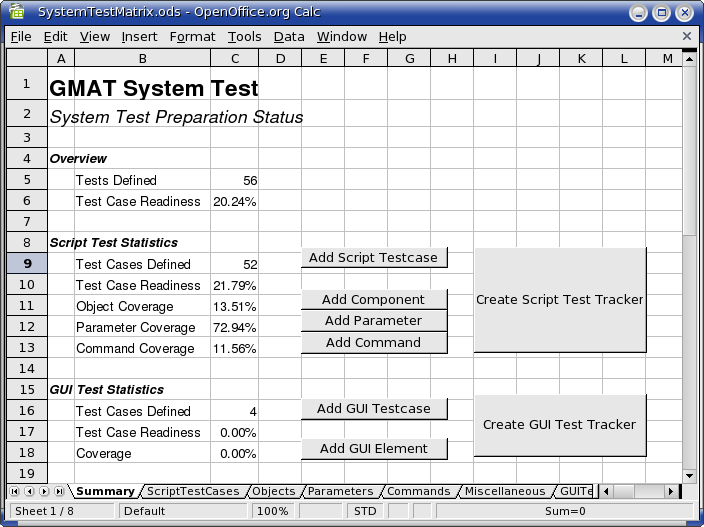
\includegraphics[400,300]{Images/SystemTestSummary.png}
\caption{\label{figure:SystemTestSummary}The System Test Summary Page}
\end{center}
\end{figure}

System testing is performed in three stages: test preparation, system testing (consisting of Script
based Testing and GUI Testing), and test result reporting.  The test preparation
phase, described in this chapter, is used to update the system test cases with tests covering new
capabilities of GMAT, and to add or update existing test cases based on lessons learned from
previous testing.  Procedures followed when executing the script based are described in
Chapter~\ref{chap:scripttests}.  GUI testing procedures are given in Chapter~\ref{chap:guitests}.
Both of those chapters include descriptions of the data collection for individual tests.
Chapter~\ref{chap:reporting} describes the process of accumulating the test results so that the
status of the system can be evaluated.

\section{Test Preparation}

GMAT system testing is managed from a set of OpenOffice\cite{OOo} spreadsheets.  The test case
structure and mapping between system functionality and corresponding tests is tracked using the
"SystemTestMatrix.ods" spreadsheet\footnote{All of the GMAT test tracking components are
configuration controlled.  Interested parties can obtain the current versions of these testing
artifacts by contacting one of the GMAT team leads.}. This spreadsheet contains pages identifying
detailed GMAT functionality and defined system test cases, and maps each element of functionality to
one or more test cases.

The spreadsheet includes a summary page, shown in Figure~\ref{figure:SystemTestSummary}, which
computes coverage for the elements tabulated on the detail pages.  If the tables in the spreadsheet
are up to date, then the summary page is an indicator of the readiness of the system tests.  Hence
the first task that testers perform when preparing for system testing is to update the test
matrices.  Once the test matrices have been updated, the test cases are updated to cover any new
functionality in the system.  Test preparation is finished when a complete set of test cases has
been developed, covering all of the elements in the updated test matrix tables.

\begin{figure}[htb]
\begin{center}
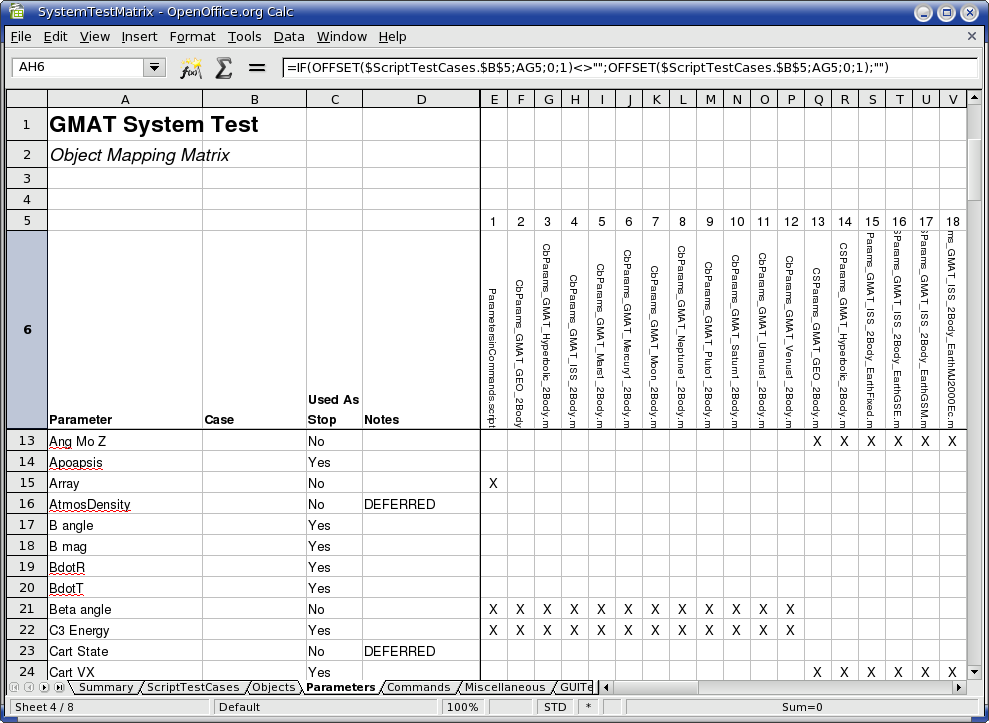
\includegraphics[400,300]{Images/ComponentTestMatrix.png}
\caption{\label{figure:ComponentTestMatrix}An Object Test Matrix}
\end{center}
\end{figure}

To summarize, when a new piece of functionality is added to GMAT that users can access, the test
team, working with the developers and users, updates the test matrices by performing three steps:

\begin{enumerate}
\item Identify and add all new elements of the system to the test matrices.
\item\label{item:planTheWork} Identify test cases that cover the new elements.  This may involve
modifying existing test cases or creating new test cases, depending on the functionality of the new
element.
\item Create or update the test cases as needed to implement the planned coverage identified in
item~\ref{item:planTheWork}.
\end{enumerate}

When these steps have been performed, the coverage matrices are up to date, and the test team is
ready to run the system test by executing all of the test cases in the matrices.  The following
paragraphs describe the procedure for executing these steps.


\section{Updating the Element Lists in the Test Matrices}

Figure~\ref{figure:ComponentTestMatrix} shows an example of the matrices used to identify GMAT's
implemented functionality.  Separate tables exist for the user accessible Components (Spacecraft,
Solvers, Propagators, and so forth), Parameters that GMAT can calculate, Commands used when defining
the mission sequence, Graphical User Interface elements (GuiElements), and miscellaneous other
configurable elements.  These tables capture a static view of every item that a user can interact
with when running GMAT.

Each table lists the configurable elements in column A, and constructs, when appropriate,
configurations and subconfigurations of those objects in columns B~(labeled ``Cases'') and
C~(``Subcases'').  Column D, ``Notes'', is used to indicate other considerations.  Elements that are
not yet scheduled for testing can be entered in the tables; when that happens, the entry in the
``Notes'' column should be set to the keyword ``DEFERRED''.

The first step in updating the test matrices is to ensure that the lists of accessible elements are
complete, capturing any new elements and configurations added to the system since the last time the
matrix was updated.  Testers have two options for performing these updates: they can either edit the
tables by hand, and check that all related formatting and equations are updated correctly, or they
can use the macros built into the spreadsheet to add the new elements.  The preferred approach is to
use the macros, because that approach ensures that the calculations performed by the tables are
correct.

\begin{figure}[htb]
\begin{center}
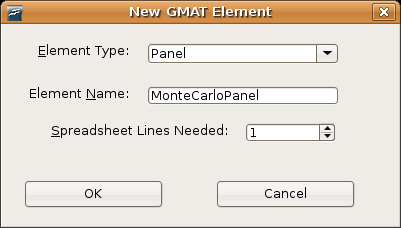
\includegraphics[200,114]{Images/AddingAnElement.png}
\caption{\label{figure:NewElement}The New Element Dialog}
\end{center}
\end{figure}

The summary page, shown in Figure~\ref{figure:ComponentTestMatrix}, for the spreadsheet contains
four buttons used to add elements to the test matrices: ``Add Resource'', ``Add Parameter'', ``Add
Command'', and ``Add GUI Element''.  When a user presses one of these buttons, a dialog box opens
that is used to set some basic information for the new element that is being tested.
Figure~\ref{figure:NewElement} shows an example of this dialog.

When this dialog is opened, users can change the type of new element being configured using the
Element Type combo box.  This option is provided in case the user selected the wrong button from the
summary page.  The user enters the name of the new element in the ElementName field.

Many of the elements that are tested can be exercised more than one way; for example, the Impulsive
Burn element can be set to run using Velocity-Normal-Binormal (VNB) delta-V vectors or a coordinate
system based delta-V vector.  Each of these modes should be tested independently, so a separate line
should exist for each on the spreadsheet.  The user reserves multiple lines on the spreadsheet by
entering the number of lines required in the ``Spreadsheet Lines Needed'' field.

After setting the data correctly on the new element dialog, the user presses the `OK'' button.  When
this action is taken, the test matrix corresponding to the type of the new element is updated. New
rows are inserted into the spreadsheet for the new element, and the formulas for the new rows are
set.  Finally, the fields that are used to calculate the test preparation statistics are updated.
If more than one row was inserted, the spreadsheet page is set to the page containing the new
element, with the active cell selected to the ``Cases'' field for the new element, so that the user
can enter the test cases required for the new element.  Each test case and subcase should be entered
at this time so that the element descriptions in the test matrix reflect the capabilities that need
to be tested.

At this point, all of the functionality in GMAT should be represented by rows in the test matrices.
The next step is to plan test cases that cover elements of the system that are not already handled
in the test suite.

\begin{figure}[h!]
\begin{center}
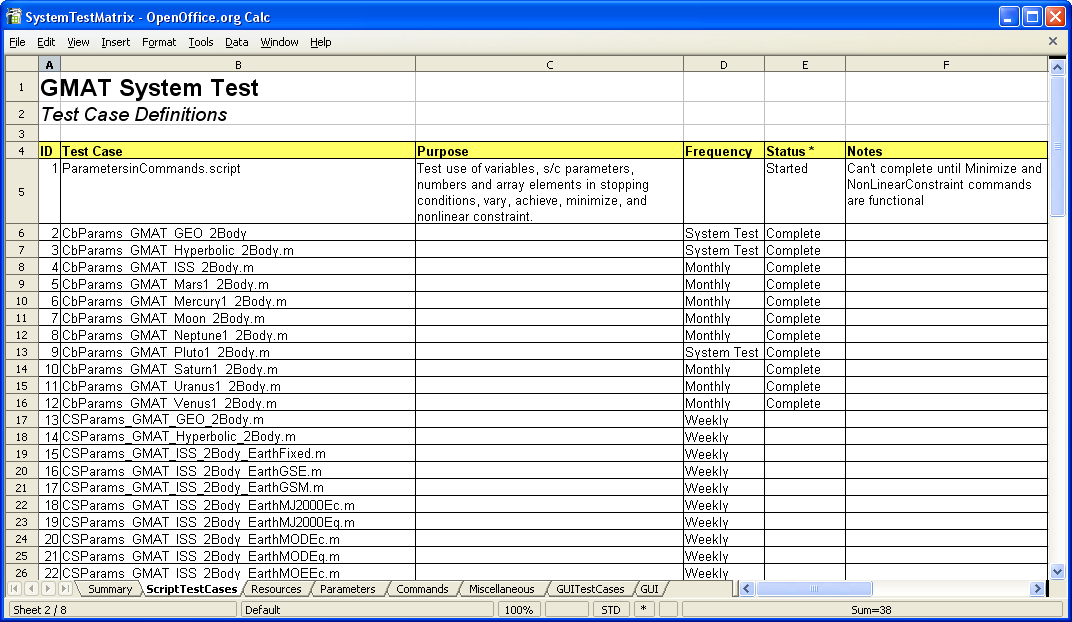
\includegraphics[460,289]{Images/TestCaseTable.png}
\caption{\label{figure:TestCaseTable}A Test Case List}
\end{center}
\end{figure}

\section{Updating the Test Case Lists}

There are two categories of test cases used in system testing GMAT, designed to exercise the system
using scripting and the graphical user interface.  When new components are added to GMAT, the test
coverage matrix is updated to exercise those new elements using the procedure described above.  This
update produces holes in the system test suite, requiring either an update of the current test cases
or the development of new test cases, depending on the nature of the new components.

The test case lists are broken into two groups: tests based on script files designed to exercise all
components used in modeling a mission, and user interface exercises designed to test the
functionality and completeness of the graphical user interface.  The test tracking spreadsheet has
separate pages for the GUI and script based test cases.  Figure~\ref{figure:TestCaseTable} shows the
page for the script cases; the GUI test case page is similar.

When a test case is added to the test case list using the spreadsheet macros described below, that
test case name is automatically picked up on the coverage tables.  Once this update has been made
and the new test cases have been added to the system test suite, users of the test matrix
spreadsheet edit the matrices to indicate the covered functionality.  In summary, the procedure for
incorporating a new test case is to perform these three steps:

\begin{enumerate}
\item \emph{Test case planning:} Identify and name the new test cases, and update the spreadsheet to
list these cases.
\item \emph{Test case writing:}  Write the new test cases, and update any older test cases that need
updating.
\item \emph{Test Matrix Mapping:}  Working from the new test cases, fill in the coverage tables for
each new or changed test case to reflect the features actually covered.
\end{enumerate}

\begin{figure}[h!]
\begin{center}
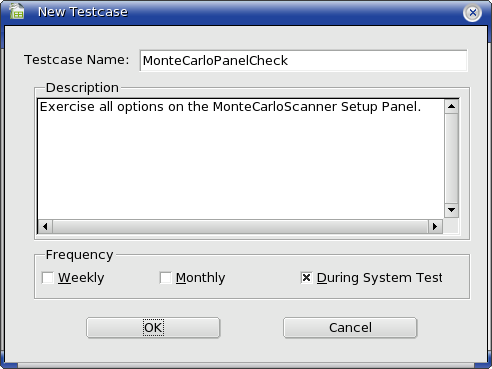
\includegraphics[246,185]{Images/AddingAGuiCase.png}
\caption{\label{figure:AddATestCase}The New Test Case Dialog}
\end{center}
\end{figure}

The procedure for adding a test case to the test case list is similar to the procedure for adding a
new element to the test matrices.  Test cases are added to the system test matrices using the ``Add
Script Testcase'' and ``Add GUI Testcase'' buttons on the summary page of the spreadsheet.  Pressing
either of these buttons opens the New Test Case dialog, shown in Figure~\ref{figure:AddATestCase}.

When a new test case has been identified, a user will open the system test spreadsheet and press the
button for the desired test case type, opening this dialog.  The user then enters the name of the
new test case.  The user enters a summary description of the test case as well to help track the
goal of the test case.  Finally, the user selects the desired frequency for execution of the test
case; cases that can be automated and run frequently, or that test critical features of the system,
should be set to run more frequently than those that are labor intensive or that test rarely used
GMAT features.

The user accepts the new test case by selecting the ``OK'' button on the spreadsheet.  When this
action is taken, several things happen in the tables in the spreadsheet.  First new test case is
added to the appropriate page of the spreadsheet, along with its descriptions and execution
frequency.  The status of the test case is set to ``Not started'', indicating that the test case
itself is not yet in the system test suite of test cases.  The new test case is added to the column
labels of the test matrices on the subsequent pages, and the formulae in in the spreadsheet are
updated to track the new tests.

This step completes the test case planning phase of the preparation process.  The next step is to
write the test cases themselves.

\section{Constructing the Test Cases}

The steps described so far ensure that there is a plan in place to test every element of GMAT for a
black box perspective.  At this point, the test cases requires for the system test have been
identified.  Next the test team needs to write the test cases, given the new functionality of the
system.  The goal for each test case is to test an integrated set of system elements when executing
a specified set of goals.

For the script based tests, this usually involves assembling a set of elements together and
performing some computations in a mission sequence.  The results of the execution of the script are
compared to known good data in order to validate that the execution behaved as expected.
Additionally, the script based testing checks to see that scripting errors are handled gracefully,
producing error messages that are clear for typical GMAT users.

GUI based scripts have similar goals.  The goals of the GUI test cases are to ensure that the GMAT
user interface lets users configure all of the elements of the system, that this configuration is
reflected in the internal components of the system, and that the user interface handles anomalous
conditions robustly.

The following paragraphs describe the approach taken to ensure that these goals are met.

\subsection{Updating Script Based Test Cases}

Script based test cases consist of a script file and validated output files generated from the
script.  All script based tests should be created from the GMAT GUI, so that any related user
interface issues can be identified during the process.  Once a scripted test has been constructed,
it should be saved with the same file name as entered in the test case table.

Each script based test should generate output in the form of a text file, using GMAT's reporting
capabilities.  Unless explicitly stated otherwise, the output file name should be the same as the
script file name with the file extension ``.report''.  The header comments on the script based tests
should indicate the following information:

\begin{itemize}
\item The first line of the script should be ``\%\% \$Id\$''.  This ensures that the CVS
version information is stored with the script.  This CVS information is the tracking identifier for
each system test case.
\item The primary elements being tested.
\item Any ancillary items that should also be examined in the execution of the test.
\item Any dependencies that need to be met to run the test successfully.  For example, the
FminconOptimizer requires a GMAT build that includes the MATLAB interfaces, a valid licensed MATLAB
executable on the test machine, and a valid licensed copy of MATLAB's Optimization Toolbox.
\item The name of the output files generated, is their name differs from the standard output file
name.
\item Whether the output data is expected to match data from previous runs.
\item Any special steps that should be taken, either prior to the run or after it completes.
\end{itemize}

\noindent A sample script test case is provided here:

\begin{quote}
\VerbatimInput[numbers=left,firstnumber=1]{./SystemTests/BasicProp.m}
\end{quote}

If a script test case fails any of the system test criteria specified in
Chapter~\ref{chap:scripttests}, the tester creates a test report summarizing the nature of the
failure.  A sample completed report is shown here:

\begin{quote}
\VerbatimInput[numbers=left,firstnumber=1]{./SystemTests/MatlabApsidesCheck.txt}
\end{quote}

\subsection{Updating the GUI Test Cases}

GUI based test cases consist of a text file describing the test.  The GUI test cases may include
additional files, depending on the nature of the test.  For example, the script reading GUI test
includes a script that needs to be read.  The purpose of the GUI tests is to validate that the
build is stable, and that the user interface panels provide complete coverage of the elements of
the system visible to the user.

The GUI test cases forms are relatively simple.  They provide, in outline form, guidelines for
testing the GUI elements.  Detailed instructions for the GUI tests are provided in
Chapter~\ref{chap:guitests}.

A sample GUI test case is provided here:

\begin{quote}
\VerbatimInput[numbers=left,firstnumber=1]{./SystemTests/ImpulsiveBurnPanel.txt}
\end{quote}

Failed GUI tests provide information about the nature of the failure durectly on the test case
form; there is no supplementary report for GUI test failures.

\section{\label{section:CompleteCoverage}Ensuring Complete System Coverage}

Once the test cases have been written, all that remains for test proparation is the confirmation
that the test cases cover all of the new features of GMAT.  This is accomplished by updating the
test matrices based on the new and revised test cases.  Each test case that has been added or
changed since the last update is collected and used to update the matrices.  For each page in the
spreadsheet containing an element to test case table, the test team needs to update the matrix
for these test cases.  The test cases are listed across the top of the matrices.  Each test case
identifies the tested elements by placing an ``X'' marker in the row corresponding to that element.
 Updated test cases should be examined to ensure that elements previously tested are still tested;
if an elemnet is no longer tested for a specific test case, the X for that element should be
removed from the matrix.

The spreadsheet contains formulas that use these markers to determine if a given element has a
corresponding test case.  The far right side of the test matrices tables accumulates this data;
every element that has at least one associated test case receives a coverage value of 1; uncovered
elements receive a coverage value of 0.  The far right side of the table also includes a column
labeled ``Row Count.'' The row count column simply counts the number of elements on the page.

\begin{figure}[htb]
\begin{center}
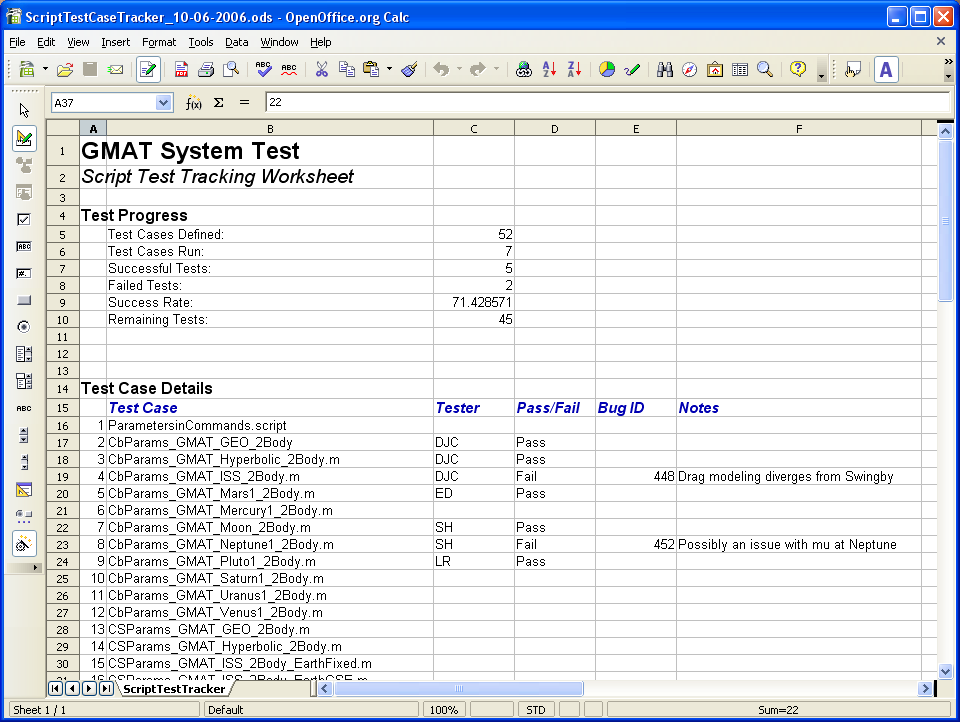
\includegraphics[460,346]{Images/TestTrackingWorksheet.png}
\caption{\label{figure:ScriptTestTracker}A Test Tracking Spreadsheet}
\end{center}
\end{figure}

The summary page examines each table in the spreadsheet and provides information about the
coverage completeness of the system tests.  Once the coverage statistics report that the elements
of the system are covered 100\%, the system tests are ready to be run.  The test team then
generates a new spreadsheet for each type of system test by pressing the ``Create Script Test
Tracker'' and ``Create GUI Test tracker'' buttons on the summary page.  These buttons generate
single page spreadsheets used to track progress through the system test.  An example is shown in
Figure~\ref{figure:ScriptTestTracker}.

This spreadsheet is used to track and report system test progress.  As each system test is
performed, the entry in the tracking spreadsheet is updated by the test team.  Examination of this
spreadsheet provides a status check on the system test.

The next two chapters provide instructions about the steps performed when running the system tests.


\chapter{\label{chap:scripttests}Executing Script Driven Tests}

The tests described in this chapter are designed to exercise all accessible objects in the core
GMAT engine, in as many combinations as is feasible.  This object coverage is performed by running
GMAT scripts designed to interact with the accessible objects from the Graphical User Interface.
Each script produces output.  The system testers examine this output, and, when possible, compare it
with the configuration managed output produced from previous runs of the scripts.  The procedure
followed when running scripted tests is documented in the sections of this chapter.

\begin{figure}[htb]
\begin{center}
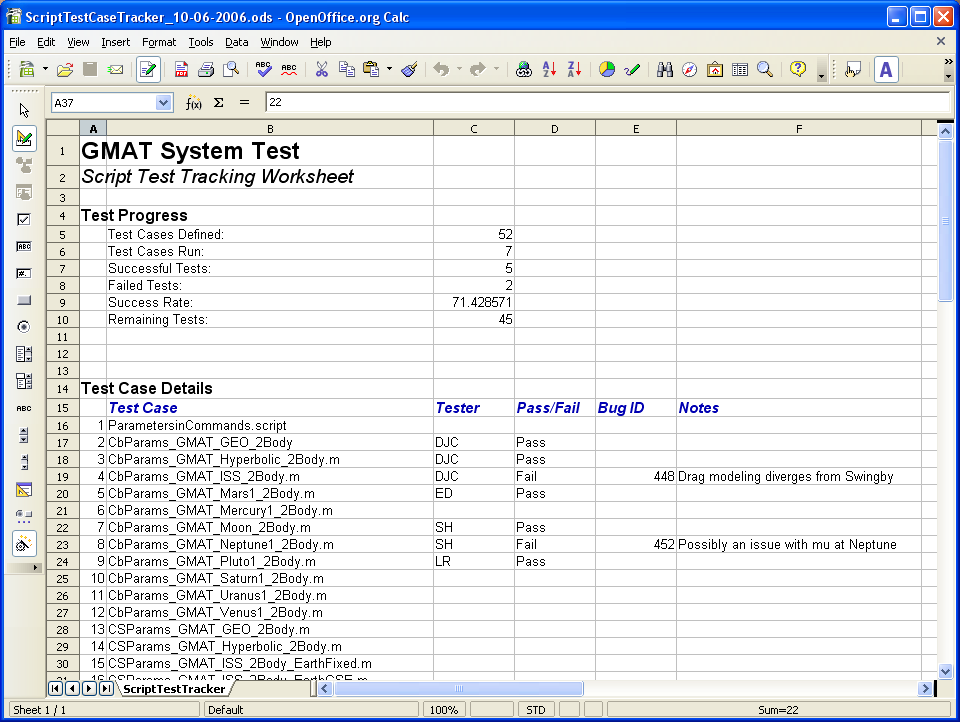
\includegraphics[460,346]{Images/TestTrackingWorksheet.png}
\caption{\label{figure:ScriptTestTracker2}The Script Test Tracking Spreadsheet}
\end{center}
\end{figure}

\section{Script Test Case Management}

The System test cases are managed from a spreadsheet generated at the conclusion of the system test
preparation process.  Figure~\ref{figure:ScriptTestTracker2} shows an example of this test
tracking spreadsheet for the script based tests\footnote{The test tracking spreadsheets, unlike the traceability matrix spreadsheet, can be saved in either OpenOffice or Excel format.}, as it looks
partway through a test cycle.

The test procedure for script based tests is relatively straightforward.  Testers follow these steps when executing the system tests:

\begin{enumerate}
\item Obtain the latest versions of the scripts and known good results from the system test repository.
\item Identify the tests each tester needs to run.
\item Open GMAT\footnote{GMAT should only be opened one time for any given testing period.  All tests run during that test period -- typically a morning or afternoon -- should be run in the same instance of GMAT.  This helps ensure that the system is stable over long periods of time.  If the system is shut down, either by the user or through a system crash, that event should be noted.}.
\item Run each test following the procedure in \ref{section:RunningScriptTests}.
\item As each test is run, record the summary results in a local copy of the test tracking
spreadsheet.
\item When anomalies are found in testing, record them local test case report files.
\item At the end of each day or when testing is finished, whichever occurs first, gather the test
case reports generated from the tests and place them in the folder used to gather the test results.
\item Close GMAT at the end of the test period.
\item At the end of each day or when testing is finished, whichever occurs first, save the local
test tracking spreadsheet with the name <spreadsheetName>\_<tester's initials> in the folder
used to gather the test results.
\item Upon completion of all assigned test cases, report that status to the system test lead.
\end{enumerate}

\section{\label{section:RunningScriptTests}Running the Scripted System Tests}

By their very nature, the GUI based tests described in Chapter~\ref{chap:guitests} follow a relatively unstructured execution sequence that mandates more structured test case documents to ensure complete system testing.  In contrast, the script based tests follow a linear execution sequence once the scripts have been written and debugged.  The rest of this chapter describes the procedure followed for the scripted tests.

\subsection{Procedure}

Each scripted test case has an associated, configuration managed script.  Most script test cases also have output data files used to compare the obtained script outputs with validated GMAT output files.  A tester follows this procedure to perform the associated system test:

\begin{enumerate}
\item Open a blank test case report file\footnote{The test case report file is only needed for
script based tests is an anomaly is found during testing.  In practice, the test case report only
needs to be opened when an anomaly is found.}.
\item Open the script in GMAT.
\item\label{item:repeatStart} Compare the resources displayed in GMAT with the resources defined in the script. Enter any anomalies in the test case report.
\item Compare the mission sequence in the script with the mission sequence displayed in GMAT.
Enter any anomalies in the test case report.
\item Run the script.
\item Examine each plot and 3D view that opens.  Enter any anomalies on the in the test case report.
\item Compare the output results from the run with the known good data.  Enter any anomalies in the test case report.
\item Press the run button.
\item Examine each plot and 3D view that opens.  Enter any anomalies on the in the test case report.
\item Compare the output results from the run with the known good data.  Enter any anomalies in the test case report.
\item\label{item:repeatEnd} Open the script in the editor window, and press the ``Build and Run''
button.
\item Examine each plot and 3D view that opens.  Enter any anomalies on the in the test case report.
\item Compare the output results from the run with the known good data.  Enter any anomalies in the test case report.
\item Save the script to a new file with the name Saved\_<Test case name>.
\item Load the saved script into GMAT.
\item Repeat steps~\ref{item:repeatStart} through~\ref{item:repeatEnd}
\item If any anomalies have been found, fill in the header and summary data on the test case
report, and save it with the file name ``<test case>\_YYYYMMDD.report'', where YYYYMMDD indicate
the year, month and day the test was run.
\end{enumerate}

\subsection{A Note on Run Frequency}

The script based tests can be run much more frequently than is feasible for the GUI tests.  Scripts that are identified as being run more frequently than at the system test frequency follow a somewhat abbreviated procedure from that defined at the system test level.  The purpose of the more frequent testing is to help catch errors in the system prior to format system testing.  Teh abbreviated test procedure performed for each weekly or monthly test is presented here:

\begin{enumerate}
\item Open the script in GMAT.
\item Run the script.
\item Examine each plot and 3D view that opens.  Report any anomalies.
\item Compare the output results from the run with the known good data.  Report any anomalies.
\item If any anomalies have been found, enter a new anomaly in the bug tracking system.
\end{enumerate}

These tests follow the full system test procedure when run as part of the system test suite.

\subsection{Reporting Results}

At the start of the system test process, a central location was established for collection of the
test results.  The final step performed by the system testers is to copy their test case worksheets and local test tracking worksheet to this central location.  This action is performed each day the
system tests are run so that the progress of the system test execution can be evaluated.  Upon
completion of all system testing by a specific tester, a final update is made and the system test
lead is notified that that tester has completed the assigned tests.  Chapter~\ref{chap:reporting}
describes the consolidation of the collected test results into a system test report.


\chapter{\label{chap:guitests}Executing Tests for the Graphical User Interface}

The tests described in this chapter are designed to exercise all of the controls and other elements
visible from the GMAT graphical user interface (GUI).  The GMAT GUI is designed to present a
consistent, easy to use interface into the underlying engine so that users of the system can view,
configure, and interact with the elements of the system during all phases of mission modeling.
System testers work with these elements, using them both to perform the expected tasks and to
attempt to perform undesired actions.  The former set of actions exercises the engine to ensure
that the system can be configured correctly.  The latter tests are run to ensure that users cannot
configure GMAT incorrectly.

\begin{figure}[htb]
\begin{center}
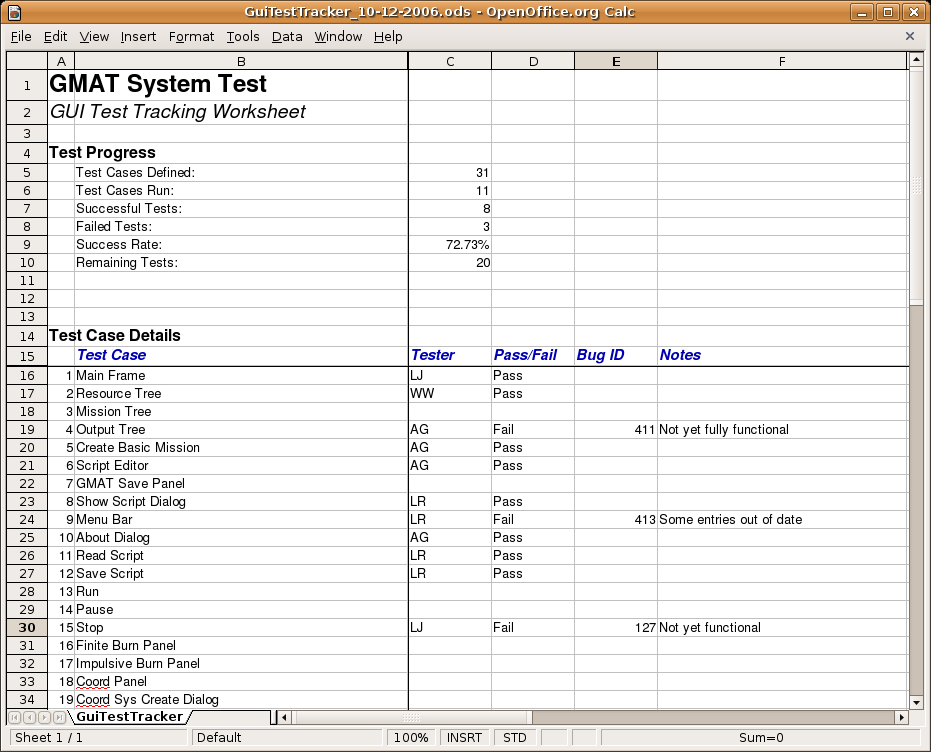
\includegraphics[460,372]{Images/GuiTestTracker.png}
\caption{\label{figure:GuiTestTracker}The GUI Test Tracking Spreadsheet}
\end{center}
\end{figure}

\section{GUI Test Case Management}

The GUI test cases are managed using a test tracking spreadsheet generated at the end of test
preparation, described in Chapter~\ref{chap:testprep}.  Figure~\ref{figure:GuiTestTracker} shows an
example of this spreadsheet partway through a testing cycle.

The test procedure for GUI based tests requires extensive exercising of the components in the GUI.
Testers follow these steps when executing the system tests:

\begin{enumerate}
\item\label{item:GetGuiTestcases} Obtain the latest versions of the GUI test cases and a local copy
of the test case tracking spreadsheet\footnote{The test tracking spreadsheet is generated from the
Systen Test Matrix spreadsheet using an OpenOffice macro, as described in
Section~\ref{section:CompleteCoverage}.}.
\item Identify the tests that the tester needs to run.
\item Open GMAT\footnote{GMAT should only be opened one time for any given testing period.  All
tests run during that test period -- typically a morning or afternoon -- should be run in the same
instance of GMAT.  This helps ensure that the system is stable over long periods of time.  If the
system is shut down, either by the user or through a system crash, that event should be noted.}.
\item Run each test following the procedure in Section~\ref{section:RunningGuiTests}.
\item As each test is run, record the results of the test on the test case worksheet retrieved in
step~\ref{item:GetGuiTestcases}.
\item When anomalies are found in testing, record them on the test case worksheet and enter them in
the bug tracking database.
\item Close GMAT at the end of the test period.
\item At the end of each day or when testing is finished, whichever occurs first, gather the
completed test case worksheets and place them in the folder used to gather the test results.
\item At the end of each day or when testing is finished, whichever occurs first, save the local
gui test tracking spreadsheet with the name <spreadsheetName>\_<tester's initials> in the folder
used to gather the test results.
\item Upon completion of all assigned test cases, report that status to the system test lead.
\end{enumerate}

The procedure for running a single test case is described next.

\section{\label{section:RunningGuiTests}Running the GUI System Tests}

By their very nature, the script based tests described in Chapter~\ref{chap:scripttests} follow a
linear execution sequence once the scripts have been written and debugged.  In contrast,
interactions performed using the GMAT GUI are less structured -- users can use the controls on the
GUI in a seemingly random fashion -- so the test cases for the GUI include allowances for
interacting with the GUI elements by the tester in a more free form manner than the script based
tests allow.

\subsection{Sample GUI Test Case}

A sample GUI test case is shown here:

\begin{quote}
\VerbatimInput[numbers=left,firstnumber=1]{./SystemTests/OpenGLPanel.txt}
\end{quote}

\begin{figure}[htb]
\begin{center}
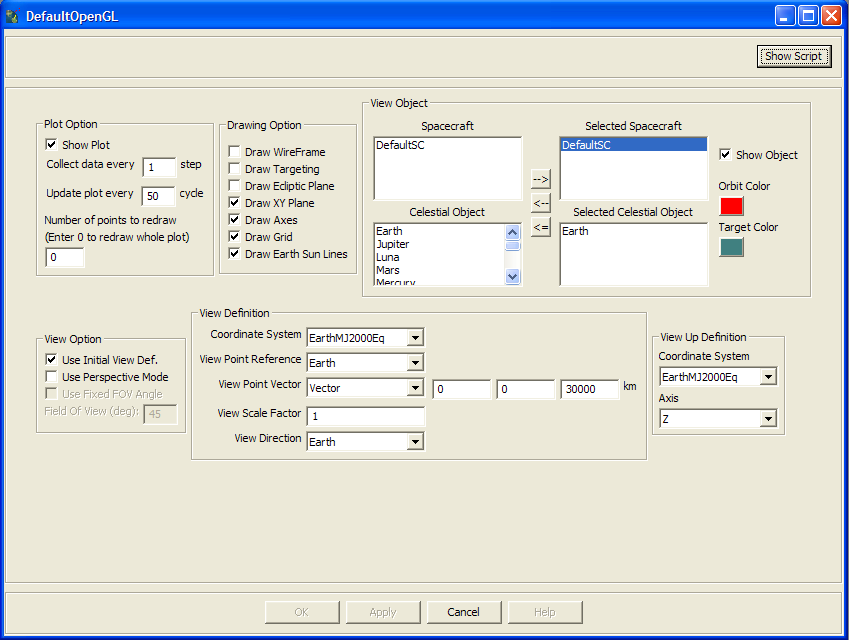
\includegraphics[300,235]{Images/OpenGLPanel.png}
\caption{\label{figure:openGLPanel}The OpenGLPlot Setup Panel}
\end{center}
\end{figure}

\noindent The test case worksheet shown here is the test case for the OpenGL plot setup panel.
The panel, shown in Figure~\ref{figure:openGLPanel}, is a fairly complex GUI panel,
containing text fields, combo boxes, check boxes, text lists, and action buttons which open color
selection dialogs.  Each element is included in the test plan worksheet, along with the standard
control processes that need to be exercised.  Each test criterion is evaluated using this worksheet,
and given a pass or fail evaluation.

\subsection{Procedure}

Each GUI test case has a worksheet like the one shown above.  A tester follows this procedure to
perform the associated system test:

\begin{enumerate}
\item Open the test case worksheet.
\item Follow the procedure outlined in the test case.
\begin{itemize}
\item Section~\ref{section:TestRules} provides detailed instructions about the process that should
be followed when testing each type of GUI element.
\item Each item identified in the worksheet is marked as either passing or failing the test.  If
the item fails, an associated bug is entered or identified in the bug tracking system and listed on
the worksheet.
\item After completing the tests on the worksheet, the tester experiments with the component for an
additional period (typically ten to fifteen minutes), checking to be sure that the component is
stable and behaves correctly when bad data is entered, and when random actions are taken using that
component.
\item Once every item on the worksheet has been evaluated and the final period of usability testing
has been performed, the number of pass and fail evaluations are counted and recorded in the
summary section of the test case worksheet. Any bugs identified on the worksheet are listed in this
section, and any additional notes that need to be recorded are also listed here\footnote{These data
are collected using an automation tool to build a status report for the system tests.}.
\end{itemize}
\item Summarize the results of the tests.
\begin{itemize}
\item Once every item on the worksheet has been evaluated, an overall pass or fail evaluation is
made and recorded in the summary section.  Any bugs identified on the worksheet are listed in this
section, and any additional notes that need to be recorded are also listed here.
\item Add the tester's name and the data the test was run to the worksheet.
\item Save the completed test case worksheet.
\end{itemize}
\item Update the local test tracking worksheet to indicate that the test was run and the results of
the run.
\item Save the test tracking worksheet.
\end{enumerate}

\subsection{Reporting Results}

At the start of the system test process, a central location was established for collection of the
test results.  The final step performed by the system testers is to copy their test case worksheets
and local test tracking worksheet to this central location.  This action is performed each day the
system tests are run so that the progress of the system test execution can be evaluated.  Upon
completion of all system testing by a specific tester, a final update is made and the system test
lead is notified that that tester has completed the assigned tests.  Chapter~\ref{chap:reporting}
describes the consolidation of the collected test results into a system test report.

\section{\label{section:TestRules}Procedural Rules}

The steps described in the preceding sections lay out the procedures followed when testing the GUI
elements of GMAT.  In this section, the criteria that must be evaluated are defined for these
tests.

\subsection{\label{Sec:GeneralTests}Test Procedures for All Elements}


%  This is the list of tests associated with panel aesthetics
\noindent\textbf{Aesthetics}\\

\noindent Description:  This set of tests is to verify look and feel
of a panel.

%
\begin{itemize}
    \item Can all of the data input fields be seen at the default panel
    size for all tabs on panel?  This includes bounding boxes.
    %
    \item Is there too much blank space surrounding the data area?
    %
    \item Is there too little blank space surrounding the data area?
    %
    \item Can the window be resized so that the data cannot be seen?
    %
\end{itemize}
\vspace{.25 in}

%
\noindent\textbf{General Panel Functionality}\\

\noindent Description:  This is the list of tests associated with
basic  panel functionality: open, close, rename, minimize, ok,
cancel, help, show script, command summary.

\begin{itemize}
    %
    \item From the appropriate tree (Resource or Mission), can you create a new object of the type being tested?
    %
    \item Can you double left click and open the panel of the new
    object?
    %
    \item Can you rename the new object?
    %
    \item If there is a default object of the type being tested, can you rename
    it?  Check at least one place in the mission sequence or resource tree to
    ensure the new name is being used.
    %
    \item Can you make a minor change on the panel, hit ok, and then rename the object?
    %
    \item Can you make a minor change on the panel, hit ok, reopen,
    and see that the change was saved?
    %
    \item Can you make a minor change on the panel, hit apply, then
    hit show script to see that the apply button saved the change
    and  it is visible in the script?
    %
    \item Can you open the panel, and while the panel is open,
    change the name in the resource tree.  Check at least one place in the mission sequence or resource tree to
    ensure the new name is being used.
    %
    \item Can you open the panel and hit cancel and the panel
    closes?
    %
    \item Can you open the panel, make a minor change in the data,
    hit cancel, reopen the panel and confirm the data was not saved?
    %
    \item Can you open the panel and
    click the small ``x" button in the upper right hand corner and close the panel?
    %
    \item Can you open the panel, make a minor change in the panel,
    click the small x button in the upper left hand corner, and be
    prompted to save data before closing?
    %
    \item When you click the minimize icon does the panel minimize?
    %
    \item When the panel is minimized, can you hit the maximize icon
     and the panel reopens to previous size?
    %
    \item When the panel is open and you use the tab key to
    negotiate panel, does the action agree with style and GUI
    philosophy?
\end{itemize}
\vspace{.25 in}

%
\noindent\textbf{Panel Data Element Completeness and Correctness}\\

\noindent Description: This set of tests verifies that all data
elements that should appear on the panel indeed appear on the panel.
It also tests that all elements that should appear in show script
appear there and that items that should not appear in show script do
not appear there.

\begin{itemize}
    %
    \item Verify that only data elements that occur in the Range
    Test Plan appear in show script and that the user does not see
    any other object fields.   Also check that defaults agree with
    Range Test Plan.
    %
    \item Verify that all elements that should appear in show script
    appear.  (See range test plan)
    %
    \item  Verify that all data elements
    that appear in Show Script also appear on the GUI.  This
    means that if you can set something in the script, ensure that it
    appears in the GUI.
    %
\end{itemize}
\vspace{.25 in}


\subsection{Procedures for Specific Control Types}
The following table provides additional guidelines that should be followed when testing each
specific type of control.
 \begin{longtable}{p{1.25 in} |p{4.5 in} }
 \caption
 [Tests for Data Objects on All Panels]
 {Tests for Data Objects on All Panels \label{Table:DataElementTests}}\\
 \hline\hline
% \multicolumn{2}{@{*}c@{*}}%
%      {This part appears at the top of the table}\\
 Element Type & Tests\\
 \hline
 \endfirsthead
 \caption[]{(Tests for Data Objects on All Panels...continued)}\\
 \hline\hline
 Element Type & Tests\\
 \hline\hline
 \endhead
 \hline
 % This goes at the&bottom.\\
 \hline
 \endfoot
 \hline
 \hline
 \endlastfoot
%-----------------------------------------------------------------------
%-----------------------Begin Table Here--------------------------------
%-----------------------------------------------------------------------
% ---- Column 1--------%
Check Boxes &
% ---- Column 2--------%
\begin{itemize} \vspace{-.25 in}
\item Set all check boxes to off (unchecked), hit show script, and verify that the functionality is
indeed turned off for each radio button and check box.
%
\item Set all check buttons to on (checked), hit apply, and show script
and verify that the functionality is indeed turned on for each radio
button and check box.
\end{itemize} \\
\hline
% ---- Column 1--------%
Radio Buttons &
% ---- Column 2--------%
\begin{itemize} \vspace{-.25 in}
   \item For each radio button on panel, select the button, and ensure that it activates
   and all others are deactivated.  Hit Apply, and then check show
   script to ensure that the configuration was properly saved.
\end{itemize} \\
\hline
%-------------- This is the beginning of a new row!!!----------------------
% ---- Column 1--------%
Combo Boxes &
% ---- Column 2--------%
\begin{itemize} \vspace{-.25 in}
\item  For each combo box on the panel, ensure that all options that
appear in Range Test Plan appear in the pull down menu.
%
\item  For each Combo box on the panel, select each allowable option, hit apply and show script
and check to see that the option was correctly saved.
%
\item Check to ensure that the combo box is not editable.
\end{itemize} \\
\hline
%-------------- This is the beginning of a new row!!!----------------------
% ---- Column 1--------%
Text Fields &
% ---- Column 2--------%
\begin{itemize} \vspace{-.2 in}
\item For each text field enter ``DNE" and ensure that if GMAT should reject this string that the string is
rejected. ( Currently, this is not an acceptable value for any GMAT
field unless the user has created an appropriate object type and
named it DNE, and is using it correctly in the GUI. )
%
\item Perform all range tests as described in Range Test Plan.
%
\item For all numeric fields, enter an allowed numeric value, hit
apply and show script and check that the value was saved.
%
\item If user-defined objects can appear in the combo box, create
one object for all allowable object types for the particular combo
box, and ensure that it appears in the combo box.  Also, hit apply
and ensure that each case appears in show script.
%
\end{itemize} \\
\hline
%-------------- This is the beginning of a new row!!!----------------------
% ---- Column 1--------%
Action Buttons &
% ---- Column 2--------%
\begin{itemize} \vspace{-.2 in}
\item For each button ensure that clicking on the button brings up the appropriate panel.
\item For the panel opened up, perform all tests defined in Section \ref{Sec:GeneralTests} and Table \ref{Table:DataElementTests}
\end{itemize} \\
\hline
%-------------- This is the beginning of a new row!!!----------------------
% ---- Column 1--------%
Selection Lists &
% ---- Column 2--------%
\begin{itemize} \vspace{-.2 in}
\item First Item
\item Second Item
\end{itemize} \\
\hline

%-------------- This is the beginning of a new row!!!----------------------
% ---- Column 1--------%
Tabbed Panels &  % ---- Column 2--------%
\begin{itemize} \vspace{-.2 in}
\item First Item
\item Second Item
\end{itemize} \\
\end{longtable}


%% ---- Column 2--------%
%\begin{itemize} \vspace{-.2 in}
%\item First Item
%\item Second Item
%\end{itemize} \\
%\hline


\subsection{Usability Testing}

The tests described in the preceding paragraphs are meant to exercise all of the elements of the
graphical user interface.  One important aspect of the interface not covered by those tests is the
usability of the system: the GUI may perform error free as designed, and still be difficult to use
in practice.  Usability testing is performed to capture information about this aspect of the GUI.



\chapter{\label{chap:reporting}Reporting and Reviewing Test Results}

This chapter describes the process followed for tracking the state of the system test process and for reporting the results of the testing.

\section{\label{section:TestStatus}System Test Status}

The status of the system tests is tracked using the Script and GUI test tracking spreadsheets described in Chapters~\ref{chap:scripttests} and~\ref{chap:guitests}.  System testers update their copies of these spreadsheet daily during system testing.  Once a week or upon request, the system test lead consolidates these spreadsheets, collecting the test results in master system test spreadsheets that can be reviewed by interested parties.

\section{\label{section:TestReport}The System Test Report}

At the conclusion of system test cycle, the reports generated during system test are consolidated into a single document.  This document is prepared using the following outline:

\renewcommand\theenumi   {\Roman{enumi}}
\renewcommand\theenumii  {\Alph{enumii}}
\renewcommand\labelenumii{\theenumii.}
\begin{enumerate}
\item Overview
\begin{enumerate}
\item Executive Summary
\item Test Results
\item Recommendations
\end{enumerate}
%%% Script Test Results
\item Script Test Case Results
\begin{enumerate}
\item Test Result Statistics
\item Summary of Failed Tests (if any)
\item Test Results
\begin{enumerate}
\item ParametersinCommands Test Case Report
\item CbParams\_GMAT\_GEO\_2Body Test Case Report\\
...
\end{enumerate}
\end{enumerate}
%%% GUI Test Results
\item GUI Test Case Results
\begin{enumerate}
\item Test Result Statistics
\item Summary of Failed Tests (if any)
\item Test Results
\begin{enumerate}
\item Mainframe Test Case Worksheet
\item Resource Tree Test Case Worksheet\\
...
\end{enumerate}
\end{enumerate}
\end{enumerate}

\section{\label{section:TestReview}System Test Review}

The final step in the system test process is to perform a review of the test results.  In preparation for this review, each team member and reviewer reviews the System Test Report, highlighting any issues that raise concerns.  These parties then meet and discuss the findings of the system testing.  The outcome of this review is a list of action items, assigned to specific individuals or teams, and a recommendation about the status of the system for release.  

A typical release recommendation will fall into one of three categories: (1) GMAT is ready for release, (2) GMAT is ready for release, contingent on specific items being addressed and approved prior to that release, or (3) GMAT is not ready for release, and needs to meet specific items and be reviewed again before release will be approved.

Following this review, a summary documenting the findings of the review is written and provided to all team members and interested parties.  Once GMAT has been released as an open source project, a public version of this summary is made available with the other project artifacts.


\part{Tests}

\chapter{Test Procedures} \label{Ch:TestProcedures}

\section{Spacecraft Orbit Tab}
\begin{table}[htbp!]
\centering
      \begin{tabular}{|p{1.05 in} |p{4.75 in} |}
      \hline
         \rowcolor[rgb]{0.8,0.8,0.8} Name & STC-3 Orbit GUI Behavior for Disallowed Conversion\\
         \hline
         Requirements & FR-1.3\\  \hline
         Summary &
         %======================  BEGIN: The Test Summary
         This  case tests GUI behavior when attempting to convert to a Keplerian state
         when the coordinate system does not have a celestial body (i.e. mu value) at the origin.
         %======================  END: The Test Summary
         \\     \hline
         PreConditions & BS-2\\     \hline
         Steps &
         %====================== BEGIN: The test procedure
         \begin{compactenum}
             \item Load BS-2.
             \item Open the dialog box for DefaultSC.
             \item Change the StateType to Keplerian.
             \item Click on the down arrow on the Coordinate System drop-down menu and inspect the available Coordinate Systems.
             \item Change the StateType to Modified Keplerian.
             \item Click on the down arrow on the Coordinate System drop-down menu and inspect the available Coordinate Systems.
             \item Change the StateType to Equinoctial.
             \item Click on the down arrow on the Coordinate System drop-down menu and inspect the available Coordinate Systems.
         \end{compactenum}
         %====================== END: The test procedure
         \\ \hline
         Expected Results & The only coordinate systems available in the inspection steps above should be EarthMJ2000Eq, EarthMJ2000Ec, and Earth Fixed.   Coordinate Systems CS\_ESL2  and  CS\_SSBary are NOT available because these orbit state representations are only valid for coordinate systems with a central body at the origin.\\
      \hline
\end{tabular}
      \label{Table: STC-3}
      \caption{STC-3 Orbit GUI Behavior for Disallowed Conversion}
      \index{Test Data!STC-3}
\end{table} 
\begin{table}[htbp!]
\centering
      \begin{tabular}{|p{1.05 in} |p{4.75 in} |}
      \hline
         \rowcolor[rgb]{0.8,0.8,0.8} Name & STC-4 Conversion to Disallowed Coordinate System from Keplerian-type Elements \\
         \hline
         Requirements & FR-1.3\\  \hline
         Summary &
         %======================  BEGIN: The Test Summary
         This  case tests GUI behavior when attempting to convert to a new coordinate system that does
         not have a celestial body at the center.
         %======================  END: The Test Summary
         \\     \hline
         PreConditions & BS-2\\     \hline
         Data &
         %====================== BEGIN: The test procedure
         \begin{compactenum}
             \item Load BS-2.
             \item Open the dialog box for DefaultSC.
             \item Change the Coordinate System to CS\_ESL2.
             \item Click on the down arrow on the State Type drop-down menu and inspect the available State Types.
             \item Change the Coordinate System to CS\_SSBary.
             \item Click on the down arrow on the State Type drop-down menu and inspect the available State Types.
         \end{compactenum}
         %====================== END: The test procedure
         \\ \hline
         Expected Results & The only State Types available are Cartesian, SphericalRADEC, and SphericalAZFPA.   State Types Keplerian, Modified Keplerian, and Equinoctial are NOT available because these orbit state representations are only valid for coordinate systems with a central body at the origin.\\
      \hline
\end{tabular}
      \label{Table: STC-4}
      \caption{STC-4 Conversion to Disallowed Coordinate System from Keplerian-type Elements }
      \index{Test Data!STC-4}
\end{table} 
\begin{table}[htbp!]
\centering
      \begin{tabular}{|p{1.05 in} |p{4.75 in} |}
      \hline
         \rowcolor[rgb]{0.8,0.8,0.8} Name & STC-5 GUI Epoch and State Independence for Time Dependent Coordinate System\\
         \hline
         Requirements & FR-1.3\\  \hline
         Summary &
         %======================  BEGIN: The Test Summary
         This test is to verify that changing the epoch of the spacecraft, does not effect
         the orbit state, even when the coordinate system is, for example, a libration point
         coordinate system that has a time varying origin and axis system.
         %======================  END: The Test Summary
         \\     \hline
         PreConditions & BS-2\\
         \hline
         Steps &
         %====================== BEGIN: The test procedure
         \begin{compactenum}
              \item Load BS-2
              \item Open the dialog box for DefaultSC
              \item Change the CoordinateSystem to CS\_ESL2
              \item Change the Epoch Format to UTCGregorian
              \item Change the Epoch value to 01 Jan 2010 12:00:00.000
              \item Hit Ok to close the dialog box
              \item Reopen the dialog box for DefaultSC.
         \end{compactenum}
         %====================== END: The test procedure
         \\\hline
         Expected Results &  The data in the GUI should agree with the data below to at least 12 significant figures.
         \begin{compactitem}
         \item DefaultSC.X =  273083.6097699367 ;
         \item DefaultSC.Y = -1332500.504835084;
         \item DefaultSC.Z = -576402.9744365886 ;
         \item DefaultSC.VX = 0.2990482122160891;
         \item DefaultSC.VY = 7.400368588891073;
         \item DefaultSC.VZ = 1.021835464804587 ;
                   
         \end{compactitem}\\
      \hline
\end{tabular}
      \label{Table: STC-5}
      \caption{STC-5 GUI Epoch and State Independence for Time Dependent Coordinate System}
      \index{Test Data!STC-5}
\end{table} 



\begin{table}[htbp!]
\centering
      \begin{tabular}{|p{1.05 in} |p{4.75 in} |}
      \hline
         \rowcolor[rgb]{0.8,0.8,0.8} Name & STC-6 Anomaly Type Change Disallowed When State is Ill-Defined\\  \hline
         Requirements & FRR-1.1\\  \hline
         Summary &
         %======================  BEGIN: The Test Summary
         If the Keplerian state definition is defined with SMA $<$ 0 and 0 $<$ ECC $<$ 1, then
         the Keplerian state is not self consistent and the user should not be able
         to change the Anomaly Type.
         %======================  END: The Test Summary
         \\     \hline
         PreConditions & BS-1\\   \hline
         Steps &
         %====================== BEGIN: The test procedure
         \begin{compactenum}
            \item Open the dialog box for DefaultSC
            \item Set the SMA to -10000
            \item Set the ECC to 1.5
            \item Click on the Anomaly Type arrow in the drop-down menu and select Eccentric Anomaly
         \end{compactenum}
         %====================== END: The test procedure
         \\ \hline
         Expected Results & You should get the following message \\      \hline
\end{tabular}
      \label{Table: TC-6}
      \caption{STC-6 Anomaly Type Change Disallowed When State is Ill-Defined}
      \index{Test Data!TC-6}
\end{table} 
\begin{table}[htbp!]
\centering
      \begin{tabular}{|p{1.05 in} |p{4.75 in} |}
      \hline
         \rowcolor[rgb]{0.8,0.8,0.8} Name & STC-7 GUI Hyperbolic Anomaly Should be Disallowed for ECC $<$ 1\\   \hline
         Requirements & FRR-1.1 \\  \hline
         Summary &
         %======================  BEGIN: The Test Summary
         This test checks that the user cannot select hyperbolic anomaly as an input for
         elliptic orbits.
         %======================  END: The Test Summary
         \\     \hline
         PreConditions & BS-1 \\  \hline
         Steps &
         %====================== BEGIN: The test procedure
         \begin{compactenum}
             \item Open the dialog box for DefaultSC
             \item Change the State Type to Keplerian
             \item Click on the down arrow in the AnomalyType drop-down menu
         \end{compactenum}
         %====================== END: The test procedure
         \\ \hline
         Expected Results & Only True Anomaly, Mean Anomaly, and Eccentric Anomaly should be
         available because the orbit is eccentric.
         \\  \hline
      \end{tabular}
      \label{Table: STC-7}
      \caption{STC-7 GUI Hyperbolic Anomaly Should be Disallowed for ECC $<$ 1}
      \index{Test Data!STC-7}
\end{table} 
\begin{table}[htbp!]
\centering
      \begin{tabular}{|p{1.05 in} |p{4.75 in} |}
      \hline
         \rowcolor[rgb]{0.8,0.8,0.8} Name & STC-8 Orbit GUI Behavior for Circular, Inclined Orbit\\
         \hline
         Requirements & FR-1.3\\  \hline
         Summary &
         %======================  BEGIN: The Test Summary
         This  case tests GUI behavior when attempting to convert to element representations when the
         cartesian state results in a circular, equatorial orbit.
         %======================  END: The Test Summary
         \\     \hline
         PreConditions & BS-1 and TD-6\\     \hline
         Data &
         %====================== BEGIN: The test procedure
         \begin{compactenum}
             \item Load BS-1.
             \item Open the dialog box for DefaultSC.
             \item Enter the Cartesian state data from TD-6.
             \item Hit Apply.
             \item Change the state to Keplerian and verify the numeric data with TD-6.
             \item Change the state to Modified Keplerian and verify the numeric data with TD-6.
             \item Change the state to SphericalRADEC and verify the numeric data with TD-6.
             \item Change the state to SphericalAZEL and verify the numeric data with TD-6.
             \item Change the state to Equinoctial and verify the numeric data with TD-6.
         \end{compactenum}
         %====================== END: The test procedure
         \\ \hline
         Expected Results & The truth data is contained in TD-6.\\
      \hline
      \end{tabular}
      \label{Table:STC-8}
      \caption{STC-8 Orbit GUI Behavior for Circular, Inclined Orbit}
      \index{Test Data!STC-8}
\end{table} 






\begin{table}[htbp!]
\centering
      \begin{tabular}{|p{1.05 in} |p{4.75 in} |}
      \hline
         \rowcolor[rgb]{0.8,0.8,0.8} Name & STC-9 Changing Anomaly Type in GUI (Eccentric Orbit)\\    \hline
         Requirements & FRR-1.1 \\  \hline
         Summary &
         %======================  BEGIN: The Test Summary
         This tests numerics of anomaly conversion via GUI for eccentric orbit.
         %======================  END: The Test Summary
         \\  \hline
         PreConditions & BS-1\\
         \hline
         Steps &
         %====================== BEGIN: The test procedure
         \begin{compactenum}
             \item Open the dialog box for DefaultSC
             \item Change SMA to 10000 km
             \item Change ECC to 0.1
             \item Change TA to 45.0 deg.
             \item Change the Anomaly Type to Mean Anomaly and compare to data below.
             \item Change the Anomaly Type to Eccentric Anomaly and compare to data below.
         \end{compactenum}
         %====================== END: The test procedure
         \\ \hline
         Expected Results & Mean anomaly is XXX.  Eccentric Anomaly is XXX \\ \hline
\end{tabular}
      \label{Table: STC-9}
      \caption{STC-9 Changing Anomaly Type in GUI (Eccentric Orbit)}
      \index{Test Data!STC-9}
\end{table} 








\begin{table}[htbp!]
\centering
      \begin{tabular}{|p{1.05 in} |p{4.75 in} |}
      \hline
         \rowcolor[rgb]{0.8,0.8,0.8} Name & STC-10 Orbit GUI Behavior for orbit with zero position\\
         \hline
         Requirements & FR-1.3\\  \hline
         Summary &
         %======================  BEGIN: The Test Summary
         This  case tests GUI behavior when attempting to convert to element representations when the
         cartesian state results in a circular, equatorial orbit.
         %======================  END: The Test Summary
         \\     \hline
         PreConditions & BS-1\\     \hline
         Data &
         %====================== BEGIN: The test procedure
         \begin{compactenum}
             \item Load BS-1.
             \item Open the dialog box for DefaultSC.
             \item Enter the following Cartesian State data:
                      \begin{compactenum}
                         \item X = 0.0
                         \item Y = 0.0
                         \item Z = 0.0
                         \item VX = 7.0;
                         \item VY = 7.0;
                         \item VZ = 7.0;
                      \end{compactenum}
             \item Hit Apply.
             \item Change the state to Keplerian and verify that the following error message is returned: The orbit is a singular conic section and the Keplerian elements are undefined.
             \item Change the state to Modified Keplerian and verify that the following error message is returned: The orbit is a singular conic section and the Modified Keplerian elements are undefined.
             \item Change the state to SphericalRADEC and verify that the following error message is returned: The orbit is a singular conic section and the SphericalRADEC elements are undefined.
             \item Change the state to SphericalAZEL and verify that the following error message is returned: The orbit is a singular conic section and the SphericalAZEL elements are undefined.
             \item Change the state to Equinoctial and verify that the following error message is returned:
                   The orbit is a singular conic section and the Equinoctial elements are undefined.
         \end{compactenum}
         %====================== END: The test procedure
         \\ \hline
         Expected Results & The truth data is described above.\\
      \hline
      \end{tabular}
      \label{Table:STC-10}
      \caption{STC-10 Orbit GUI Behavior for orbit with zero position}
      \index{Test Data!STC-10}
\end{table} 






\begin{table}[htbp!]
\centering
      \begin{tabular}{|p{1.05 in} |p{4.75 in} |}
      \hline
         \rowcolor[rgb]{0.8,0.8,0.8} Name & STC-11 Orbit State Conversion for Orbit with Zero State\\
         \hline
         Requirements & FR-1.3\\  \hline
         Summary &
         %======================  BEGIN: The Test Summary
         This  case tests GUI behavior when attempting to convert to element representations when the
         cartesian state results in a circular, equatorial orbit.
         %======================  END: The Test Summary
         \\     \hline
         PreConditions & BS-1\\     \hline
         Data &
         %====================== BEGIN: The test procedure
         \begin{compactenum}
             \item Load BS-1.
             \item Open the dialog box for DefaultSC.
             \item Enter the following Cartesian State data:
                      \begin{compactenum}
                         \item X = 0.0
                         \item Y = 0.0
                         \item Z = 0.0
                         \item VX = 0.0;
                         \item VY = 0.0;
                         \item VZ = 0.0;
                      \end{compactenum}
             \item Hit Apply.
             \item Change the state to Keplerian and verify that the following error message is returned: The orbit is a singular conic section and the Keplerian elements are undefined.
             \item Change the state to Modified Keplerian and verify that the following error message is returned: The orbit is a singular conic section and the Modified Keplerian elements are undefined.
             \item Change the state to SphericalRADEC and verify that the following error message is returned: The orbit is a singular conic section and the SphericalRADEC elements are undefined.
             \item Change the state to SphericalAZEL and verify that the following error message is returned: The orbit is a singular conic section and the SphericalAZEL elements are undefined.
             \item Change the state to Equinoctial and verify that the following error message is returned:
                   The orbit is a singular conic section and the Equinoctial elements are undefined.
         \end{compactenum}
         %====================== END: The test procedure
         \\ \hline
         Expected Results & The truth data is described above.\\
      \hline
      \end{tabular}
      \label{Table:STC-11}
      \caption{STC-11 Orbit State Conversion for Orbit with Zero State}
      \index{Test Data!STC-11}
\end{table} 





\begin{table}[htbp!]
\centering
      \begin{tabular}{|p{1.05 in} |p{4.75 in} |}
      \hline
         \rowcolor[rgb]{0.8,0.8,0.8} Name & STC-12 Orbit GUI behavior when performing Modulo on Keplerian Angular Elements\\
         \hline
         Requirements & FR-1.3\\  \hline
         Summary &
         %======================  BEGIN: The Test Summary
         This  case tests GUI behavior when attempting to convert to element representations when the
         cartesian state results in a circular, equatorial orbit.
         %======================  END: The Test Summary
         \\     \hline
         PreConditions & BS-1\\     \hline
         Data &
         %====================== BEGIN: The test procedure
         \begin{compactenum}
             \item Load BS-1.
             \item Open the dialog box for DefaultSC.
             \item Change the State Type to Keplerian
             \item Change INC to 370.0 degrees.
             \item Change RAAN to 380.0 degrees.
             \item Change AOP to 390.0 degrees.
             \item Change TA t0 400.0 degrees.
             \item Change the State Type to Cartesian.
             \item Change the State Type to Keplerian.
         \end{compactenum}
         %====================== END: The test procedure
         \\ \hline
         Expected Results & INC = 10.0 degrees, RAAN = 20 degrees, AOP = 30.0 degrees, and TA = 40.0 degrees. (All
         values match to 14 sig. figs.)\\
      \hline
      \end{tabular}
      \label{Table:STC-12}
      \caption{STC-12 Orbit GUI behavior when performing Modulo on Keplerian Angular Elements}
      \index{Test Data!STC-12}
\end{table} 

\begin{table}[htbp!]
\centering
      \begin{tabular}{|p{1.05 in} |p{4.75 in} |}
      \hline
         \rowcolor[rgb]{0.8,0.8,0.8} Name & STC-13 Orbit GUI behavior when performing Modulo on Modified Keplerian Angular Elements\\
         \hline
         Requirements & FR-1.3\\  \hline
         Summary &
         %======================  BEGIN: The Test Summary
         This  case tests GUI behavior when attempting to convert to element representations when the
         cartesian state results in a circular, equatorial orbit.
         %======================  END: The Test Summary
         \\     \hline
         PreConditions & BS-1\\     \hline
         Data &
         %====================== BEGIN: The test procedure
         \begin{compactenum}
             \item Load BS-1.
             \item Open the dialog box for DefaultSC.
             \item Change the State Type to Modified Keplerian
             \item Change INC to 370.0 degrees.
             \item Change RAAN to 380.0 degrees.
             \item Change AOP to 390.0 degrees.
             \item Change TA t0 400.0 degrees.
             \item Change the State Type to Cartesian.
             \item Change the State Type to Keplerian.
         \end{compactenum}
         %====================== END: The test procedure
         \\ \hline
         Expected Results & INC = 10.0 degrees, RAAN = 20 degrees, AOP = 30.0 degrees, and TA = 40.0 degrees. (All
         values match to 14 sig. figs.)\\
      \hline
      \end{tabular}
      \label{Table:STC-13}
      \caption{STC-13 Orbit GUI behavior when performing Modulo on Modified Keplerian Angular Elements}
      \index{Test Data!STC-13}
\end{table} 

\begin{table}[htbp!]
\centering
      \begin{tabular}{|p{1.05 in} |p{4.75 in} |}
      \hline
         \rowcolor[rgb]{0.8,0.8,0.8} Name & STC-14 Orbit GUI behavior when performing Modulo on SphericalRADEC Angular Elements\\
         \hline
         Requirements & FR-1.3\\  \hline
         Summary &
         %======================  BEGIN: The Test Summary
         This  case tests GUI behavior when attempting to convert to element representations when the
         cartesian state results in a circular, equatorial orbit.
         %======================  END: The Test Summary
         \\     \hline
         PreConditions & BS-1\\     \hline
         Data &
         %====================== BEGIN: The test procedure
         \begin{compactenum}
             \item Load BS-1.
             \item Open the dialog box for DefaultSC.
             \item Change the State Type to Spherical
             \item Change RA to 370.0 degrees.
             \item Change DEC to 380.0 degrees.
             \item Change RAV to 390.0 degrees.
             \item Change DECV t0 400.0 degrees.
             \item Change the State Type to Cartesian.
             \item Change the State Type to Keplerian.
         \end{compactenum}
         %====================== END: The test procedure
         \\ \hline
         Expected Results & RA = 10.0 degrees, DEC = 20 degrees, RAV = 30.0 degrees, and DECV = 40.0 degrees. (All
         values match to 14 sig. figs.)\\
      \hline
      \end{tabular}
      \label{Table:STC-14}
      \caption{STC-14 Orbit GUI behavior when performing Modulo on SphericalRADEC Angular Elements}
      \index{Test Data!STC-14}
\end{table} 

\begin{table}[htbp!]
\centering
      \begin{tabular}{|p{1.05 in} |p{4.75 in} |}
      \hline
         \rowcolor[rgb]{0.8,0.8,0.8} Name & STC-15 Spacecraft GUI Modified Keplerian to SphericalRADEC State Conversion\\
         \hline
         Requirements & FRR-1.3\\ \hline
         Summary &
         %----------------------  The Test Summary
         This test case applies to state representation conversions performed by the Spacecraft Orbit dialog box.  \\
         \hline
         PreConditions & To run this test you need to load BS-1 and have data defined in TD-1 available.\\
         \hline
         Steps &
         %------- The test data is here
         \begin{compactenum}
         \item Open the dialog box for DefaultSC via the GUI.
         \item Change the state type to Modified Keplerian.
         \item Enter the Modified Keplerian data defined in table TD-1.
         \item Hit the apply button.
         \item Change the state type drop down box to SphercialRADEC and compare the state to the
         SphericalRADEC state data contained in TD-1. The states should be equivalent to 1significant figures.
         \end{compactenum}\\
         %------- The test data is here
         \hline
         Expected Results & The expected numeric results are described in above and in TD-1.\\
      \hline
\end{tabular}
      \label{Table: STC-15}
      \caption{STC-15 Spacecraft GUI Modified Keplerian to SphericalRADEC State Conversion}
       \index{Test Data!STC-15}
\end{table} 

\begin{table}[htbp!]
\centering
      \begin{tabular}{|p{1.05 in} |p{4.75 in} |}
      \hline
         \rowcolor[rgb]{0.8,0.8,0.8} Name & STC-16 Orbit GUI behavior when performing Modulo on Equinoctial Angular Elements\\
         \hline
         Requirements & FR-1.3\\  \hline
         Summary &
         %======================  BEGIN: The Test Summary
         This  case tests GUI behavior when attempting to convert to element representations when the
         cartesian state results in a circular, equatorial orbit.
         %======================  END: The Test Summary
         \\     \hline
         PreConditions & BS-1\\     \hline
         Data &
         %====================== BEGIN: The test procedure
         \begin{compactenum}
             \item Load BS-1.
             \item Open the dialog box for DefaultSC.
             \item Change the State Type to Spherical
             \item Change RA to 370.0 degrees.
             \item Change DEC to 380.0 degrees.
             \item Change AZI to 390.0 degrees.
             \item Change FPA t0 400.0 degrees.
             \item Change the State Type to Cartesian.
             \item Change the State Type to Keplerian.
         \end{compactenum}
         %====================== END: The test procedure
         \\ \hline
         Expected Results & RA = 10.0 degrees, DEC = 20 degrees, AZI = 30.0 degrees, and FPA = 40.0 degrees. (All
         values match to 14 sig. figs.)\\
      \hline
      \end{tabular}
      \label{Table:STC-16}
      \caption{STC-16 Orbit GUI behavior when performing Modulo on Equinoctial Angular Elements}
      \index{Test Data!STC-16}
\end{table} 

%\begin{table}[htbp!]
\centering
      \begin{tabular}{|p{1.05 in} |p{4.75 in} |}
      \hline
         \rowcolor[rgb]{0.8,0.8,0.8} Name & STC-18 Spacecraft GUI SphericalRADec to Cartesian Conversion\\
         \hline
         Requirements & FRR-1.3\\ \hline
         Summary &
         %----------------------  The Test Summary
         This test case applies to state representation conversions performed by the Spacecraft Orbit dialog box.  \\
         \hline
         PreConditions & To run this test you need to load BS-1 and have data defined in TD-1 available.\\
         \hline
         Steps &
         %------- The test data is here
         \begin{compactenum}
         \item Open the dialog box for DefaultSC via the GUI.
         \item Change the state type to SphericalRADEC.
         \item Enter the SphericalRADEC data defined in table TD-1.
         \item Hit the apply button.
         \item Change the state type drop down box to Cartesian and compare the Cartesian state to the
         Cartesian state data contained in TD-1. The states should be equivalent to 14 significant figures.
         \end{compactenum}\\
         %------- The test data is here
         \hline
         Expected Results & The expected numeric results are described above and in TD-1.\\
      \hline
\end{tabular}
      \label{Table: STC-18}
      \caption{STC-18 Spacecraft GUI SphericalRADEC to Cartesian State Conversion}
       \index{Test Data!STC-18}
\end{table} 
%\begin{table}[htbp!]
\centering
      \begin{tabular}{|p{1.05 in} |p{4.75 in} |}
      \hline
         \rowcolor[rgb]{0.8,0.8,0.8} Name & STC-19 Spacecraft GUI SphericalRADec to Keplerian Conversion\\
         \hline
         Requirements & FRR-1.3\\ \hline
         Summary &
         %----------------------  The Test Summary
         This test case applies to state representation conversions performed by the Spacecraft Orbit dialog box.  \\
         \hline
         PreConditions & To run this test you need to load BS-1 and have data defined in TD-1 available.\\
         \hline
         Steps &
         %------- The test data is here
         \begin{compactenum}
         \item Open the dialog box for DefaultSC via the GUI.
         \item Change the state type to SphericalRADEC.
         \item Enter the SphericalRADEC data defined in table TD-1.
         \item Hit the apply button.
         \item Change the state type drop down box to Keplerian and compare the Keplerian state to the
         Keplerian state data contained in TD-1. The states should be equivalent to 14 significant figures.
         \end{compactenum}\\
         %------- The test data is here
         \hline
         Expected Results & The expected numeric results are described above and in TD-1.\\
      \hline
\end{tabular}
      \label{Table: STC-19}
      \caption{STC-19 Spacecraft GUI SphericalRADEC to Keplerian State Conversion}
       \index{Test Data!STC-19}
\end{table} 
%\begin{table}[htbp!]
\centering
      \begin{tabular}{|p{1.05 in} |p{4.75 in} |}
      \hline
         \rowcolor[rgb]{0.8,0.8,0.8} Name & STC-20 Orbit State Conversion for Near Singular SphericalAZEl State \\
         \hline
         Requirements & FR-1.3\\  \hline
         PreConditions & BS-1\\     \hline
        Steps &
         %====================== BEGIN: The test procedure
         \begin{compactenum}
             \item Load BS-1.
             \item Open the dialog box for DefaultSC.
             \item Change the state type to SphercialAZFPA
             \item Set the SphercialAZFPA state to the following values
                 \begin{compactenum}
                    \item RMAG  = 7000.00000
                    \item RA = 0
                    \item DEC = -0.04094487109516581
                    \item VMAG = 10.63431419820442
                    \item AZI = 0
                    \item FPA = 0.02061675296478873
                    \end{compactenum}
             \item Hit Apply.
             \item Change state type to Keplerian and ensure that the following error is thrown: ``Warning: A nearly singular conic section was encountered while converting from the SphercialAZFPA state to the Keplerian elements so conversion was aborted.  The radius of periapsis must be greater than 1 meter."
             \item Change state type to Modified Keplerian and ensure that the following error is thrown: ``Warning: A nearly singular conic section was encountered while converting from the SphercialAZFPA state to the Modified Keplerian elements so conversion was aborted.  The radius of periapsis must be greater than 1 meter."
             \item Change state type to Equinoctial and ensure that the following error is thrown:  ``Warning: A nearly singular conic section was encountered while converting from the SphercialAZFPA state to the Equinoctial elements so conversion was aborted.  The radius of periapsis must be greater than 1 meter."
                 \item Change RMAG to 0.00001 and click apply.
                 \item Repeat steps 5, 6, and 7.
                 \item Change RMAG to 70000.
                 \item Change VMAG to 1e-14.
                 \item Repeat steps 5, 6, and 7.
                 \item Change state type to SphericalRADEC and ensure that the following error is thrown: ``Warning: A nearly singular conic section was encountered while converting from the SphercialAZFPA state to the SphericalRADEC state so conversion was aborted.  The Right Ascension and Declination of velocity are undefined."
         \end{compactenum}
         %====================== END: The test procedure
         \\ \hline
         Expected Results & Test results are described above.\\
      \hline
      \end{tabular}
      \label{Table:STC-20}
      \caption{STC-20 Orbit State Conversion for Near Singular SphericalAZEl state}
      \index{Test Data!STC-20}
\end{table}

\begin{table}[htbp!]
\centering
      \begin{tabular}{|p{1.05 in} |p{4.75 in} |}
      \hline
         \rowcolor[rgb]{0.8,0.8,0.8} Name & STC-23 Spacecraft GUI UTCGregorian to Other Epoch Types\\
         \hline
         Requirements & FRR-2.4\\ \hline
         Summary &
         %----------------------  The Test Summary
         This test case applies to epoch representation conversions performed by the Spacecraft Orbit dialog box.  \\
         \hline
         PreConditions & To run this test you need to load BS-1 and have data defined in TD-2 available.\\
         \hline
         Steps &
         %------- The test data is here
         \begin{compactenum}
         \item Open the dialog box for DefaultSC via the GUI.
         \item Change the Epoch Format to UTCGregorian.
         \item Enter the UTCGregorian epoch defined in Table \ref{Table:TD-2}.
         \item Hit the apply button.
         \item Change the Epoch Format drop down box to UTCModJulian and compare the epoch to the
          data contained in TD-2. The epoch should agree identically. 
         \end{compactenum}\\
         %------- The test data is here
		 \hline
         Alternative Paths &
         %------- The test data is here
         \begin{compactenum}
         \item Perform the test using TAIGregorian, TAIModJulian, TTGregorian, TTModJulian, A1Gregorian
         and A1ModJulian in place of UTCModJulian in step 5.
         \end{compactenum}\\
         %------- The test data is here
         \hline
         Expected Results & The expected numeric results are described above and in TD-2.\\
      \hline
\end{tabular}
      \label{Table:STC-23}
      \caption{STC-23 Spacecraft GUI UTCGregorian to Other Epoch Types}
       \index{Test Data!STC-23}
\end{table} 
\begin{table}[htbp!]
\centering
      \begin{tabular}{|p{1.0 in} |p{5.0 in} |}
         \hline
          \rowcolor[rgb]{0.8,0.8,0.8}  Name & STC-24 State conversion in the spacecraft orbit dialog box\\
         \hline
         Requirements & FRR-2.3\\ \hline
         Summary & This test case represents $n(n-1)$ tests where $n$ is the number of state representations
         supported as input types in GMAT.  Each test case is designated a unique number.  For example,
         STC-24.17 tests GUI conversion from SphericalRADEC to Keplerian elements.  The procedures described below
         must be performed for each test case in the table below.   \\ \hline
         PreConditions & To run this test you need to load BS-1 and have data defined in TD-1 available.\\ \hline
         Steps &
         %------- The test data is here
          \begin{compactenum}
             \item Select subtest number. ( STC-24.17, for example )
             \item Create a new spacecraft.
             \item Change the Epoch Format to the format defined in the first column of
                   the row containing the test case ID.  (SphericalRADEC, for STC-24.17)
             \item Enter the epoch in the Define Format from TD-1.
             \item Change the Epoch Format to the format defined in the first row of the column containing  the test case Id. (Keplerian  for STC-24.17)
             \item Verify that the new state matches the value for that format given in TD-1 to 14 significant figures.
          \end{compactenum}
          \vspace{.1 in}
          \begin{centering}
          \begin{tabular}{|l|c|c|c|c|c|c|c|c|}
          \hline
             & {\begin{sideways}\parbox{2.9cm}{Cartesian}\end{sideways}} &
             {\begin{sideways}\parbox{2.9cm}{Keplerian}\end{sideways}} &
             {\begin{sideways}\parbox{2.9cm}{Mod. Keplerian}\end{sideways}} &
             {\begin{sideways}\parbox{2.9cm}{SphericalRADEC}\end{sideways}} &
             {\begin{sideways}\parbox{2.9cm}{SphericalAZFPA}\end{sideways}}  &
             {\begin{sideways}\parbox{2.9cm}{Equinoctial}\end{sideways}}  \\ \hline
             Cartesian & N/A & 24.1 & 24.2 & 24.3 & 24.4 & 24.5\\ \hline
             Keplerian & 24.6 & N/A & 24.7 & 24.8 & 24.9 & 24.10 \\ \hline
             TAIGregorian & 25.11 & 24.12 & N/A & 24.13 & 24.14 & 24.15 \\ \hline
             SphericalRADEC & 24.16 & 24.17 & 24.18 & N/A & 24.19 & 24.20 \\ \hline
             SphericalAZFPA & 24.21 & 24.22 & 24.23 & 24.24 & N/A & 24.25 \\ \hline
             Equinoctial & 24.26 & 24.27 & 24.28 & 24.29 & 24.30 &  N/A\\ \hline
          \end{tabular}
          \end{centering} \vspace{0.1 in}\\
         %------- The test data is here
         \hline
         Expected Results & The expected numeric results are described above and in TD-1.\\
      \hline
\end{tabular}
   \label{Table:STC-24}
   \caption{STC-24 State Representation conversion in the spacecraft orbit dialog box}
    \index{Test Data!STC-24}
\end{table} 
\begin{table}[htbp!]
\centering
      \begin{tabular}{|p{1.05 in} |p{4.75 in} |}
      \hline
         \rowcolor[rgb]{0.8,0.8,0.8} Name & STC-25 Spacecraft GUI A1Gregorian to Other Epoch Types\\
         \hline
         Requirements & FRR-2.4\\ \hline
         Summary &
         %----------------------  The Test Summary
         This test case applies to epoch representation conversions performed by the Spacecraft Orbit dialog box.  \\
         \hline
         PreConditions & To run this test you need to load BS-1 and have data defined in TD-2 available.\\
         \hline
         Steps &
         %------- The test data is here
         \begin{compactenum}
         \item Open the dialog box for DefaultSC via the GUI.
         \item Change the Epoch Format to A1Gregorian.
         \item Enter the A1Gregorian epoch defined in Table \ref{Table:TD-2}.
         \item Hit the apply button.
         \item Change the Epoch Format drop down box to UTCGregorian and compare the epoch to the
          data contained in TD-2. The epoch should agree identically.
         \end{compactenum}\\
         %------- The test data is here
		 \hline
         Alternative Paths &
         %------- The test data is here
         \begin{compactenum}
         \item Perform the test using UTCModJulian, TAIGregorian, TAIModJulian, TTGregorian, TTModJulian,
         and A1ModJulian in place of UTCGregorian in step 5.
         \end{compactenum}\\
         %------- The test data is here
         \hline
         Expected Results & The expected numeric results are described above and in TD-2.\\
      \hline
\end{tabular}
      \label{Table:STC-25}
      \caption{STC-25 Spacecraft GUI A1Gregorian to Other Epoch Types}
       \index{Test Data!STC-25}
\end{table} 

\clearpage
\section{Spacecraft Attitude Tab}
\begin{table}[htbp!]
\centering
      \begin{tabular}{|p{1.0 in} |p{5.0 in} |}
         \hline
          \rowcolor[rgb]{0.8,0.8,0.8}  Name & STC-26 Attitude Conversion in the Spacecraft Attitude Dialog Box\\
         \hline
         Requirements & FRR-3.3\\ \hline
         Summary & This test case represents $n(n-1)$ tests where $n$ is the number of attitude representations
         supported as input types in GMAT.  Each test case is designated a unique number.  For example,
         STC-26.32 tests conversion from a 231 to a 232 Euler angle sequence.  The procedures described below
         must be performed for each test case in the table below.   \\ \hline
         PreConditions & To run this test you need to load BS-1 and have data defined in TD-8 available.\\ \hline
         Steps &
         %------- The test data is here
          \begin{compactenum}
             \item Select subtest number. ( STC-26.32, for example)
             \item Create a new spacecraft.
             \item Open the dialog box for the new spacecraft.
             \item Click on the Attitude tab.
             \item Change the AttitudeStateType to the format defined in the first column of
                   the row containing the test case ID.  (Euler Angles, for STC-26.32)
             \item If the AttitudeStateType is EulerAngles, change the EulerAngleSequence to the
                   sequence defined in the first column of
                   the row containing the test case ID.  (231, for STC-26.32)
             \item Enter the attitude state for the test ID using the data from TD-8.
             \item Hit Apply.
             \item Change the AttitudeStateType to the format defined in the first row of the column containing  the test case Id. (Euler Angles, for STC-26.32)
             \item If the AttitudeStateType is EulerAngles, Change the EulerAngleSequence to the format defined in the first row of the column containing  the test case Id. (232, for STC-26.32)
             \item Verify that the new epoch exactly matches the value for that format given in TD-8.
             \item Compare the new Euler Angles to those in TD-8 for the new attitude representation.  The values should agree to at least 13 significant figures.
          \end{compactenum}
          \vspace{.1 in}
          \begin{centering} \footnotesize
          \begin{tabular}{|l|c|c|c|c|c|c|c|c|c|c|c|c|c|c|c|c|c|}
          \hline
             & \rotatebox{90}{$\mathbf{q}$ } &
             \rotatebox{90}{ 123 } &
             \rotatebox{90}{ 231  }&
             \rotatebox{90}{ 312  } &
             \rotatebox{90}{ 132  } &
             \rotatebox{90}{ 321 } &
             \rotatebox{90}{ 213  }  &
             \rotatebox{90}{ 121 } &
             \rotatebox{90}{ 232  } &
             \rotatebox{90}{ 313  } &
             \rotatebox{90}{ 131  } &
             \rotatebox{90}{ 323  } &
             \rotatebox{90}{ 212  }  \\ \hline
             $\mathbf{q}$ & X & 1 & 2 & 3 & 4 & 5 & 6 & 7 & 8 & 9 & 10 & 11 & 12 \\ \hline
             123 & 13 & X & 14 & 15 & 16 & 17 & 18 & 19 & 20 & 21 & 22 & 23 & 24 \\ \hline
             231 & 25 & 26 & X & 27 & 28 & 29 & 30 & 31 & 32 & 33 & 34 &35 & 36 \\ \hline
             312 & 37 & 38 & 39 & X & 40 & 41 & 42 & 43 & 44 & 45 & 46 & 47 & 48 \\ \hline
             132 & 49 & 50 & 51 & 52 & X & 53 & 54 & 55 & 56 & 57 & 58 & 59 & 60 \\ \hline
             321 & 61 & 62 & 63 & 64 & 65 & X & 66 & 67 & 68 & 69 & 70 & 71 & 72 \\ \hline
             213 & 73 & 74 & 75 & 76 & 77 & 78 & X & 79 & 80 & 81 & 82 & 83 & 84  \\ \hline
             121 & 85 & 86 & 87 & 88 & 89 & 90 & 91 & X & 92 & 93 & 94 & 95 & 96  \\ \hline
             232 & 97 & 98 & 99 & 100 & 101 & 102 & 103 & 104 & X & 105 & 106 & 107 & 108  \\ \hline
             313 & 109 & 110 & 111 & 112 & 113 & 114 & 115 & 116  & X  & 117 & 118 & 119 & 120  \\ \hline
             131 & 121 & 122 & 123 & 124 & 125 & 126 & 127 & 128 & 129 & X & 130 & 131 & 132  \\ \hline
             323 & 133 & 134 & 135 & 136 & 137 & 138 & 139 & 140 & 141 & 142 & 143 & X & 144  \\ \hline
             212 & 145 & 146 & 147 & 148 & 149 & 150 & 151 & 152 & 153 & 154 & 155 & 156 & X  \\ \hline
          \end{tabular}
          \end{centering} \vspace{0.1 in}\\
         %------- The test data is here
         \hline
         Expected Results & The expected numeric results are described above and in TD-8.\\
      \hline
\end{tabular}
   \label{Table:STC-26}
   \caption{STC-26 Attitude Conversion in the Spacecraft Attitude Dialog Box}
    \index{Test Data!STC-26}
\end{table} 

\begin{table}[htbp!]
\centering
      \begin{tabular}{|p{1.05 in} |p{4.75 in} |}
      \hline
         \rowcolor[rgb]{0.8,0.8,0.8} Name & Attitude GUI Behavior When Entering Zero Quaternion\\
         \hline
         Requirements & FR-3.1\\  \hline
         PreConditions & BS-1\\     \hline
         Data &
         %====================== BEGIN: The test procedure
         \begin{compactenum}
             \item Load BS-1.
             \item Open the dialog box for DefaultSC.
             \item Click on the attitude tab.
             \item Set all values of the quaternion to zero.
             \item Click Ok.
         \end{compactenum}
         %====================== END: The test procedure
         \\ \hline
         Expected Results & The following warning is displayed:  The magnitude of a quaternion must be greater than 1e-10.\\
      \hline
      \end{tabular}
      \label{Table:STC-17}
      \caption{STC-17 Attitude GUI Behavior When Entering Zero Quaternion}
      \index{Test Data!STC-17}
\end{table} 
\clearpage
\section{Differential Corrector}


\begin{table}[htbp!]
\centering
      \begin{tabular}{|p{1.05 in} |p{4.75 in} |}
      \hline
         \rowcolor[rgb]{0.8,0.8,0.8} Name & TC-1 Differential Corrector Dialog Box Range Tests - Disallowed Values\\
         \hline
         Requirements & FR-19\\  \hline
         Summary &
         %======================  BEGIN: The Test Summary
         This case verifies the Differential Corrector dialog box rejects disallowed data.
         %======================  END: The Test Summary
         \\     \hline
         PreConditions & BS-1\\     \hline
         Data &
         %====================== BEGIN: The test procedure
         \begin{compactenum}
             \item Load BS-1.
             \item In the solvers folder in the mission tree, right-click on the Boundary Value Solvers folder and add a Differential Corrector.
             \item Open the dialog box for the new Differential Corrector.
             \item In the Max Iterations field, enter -2, and hit Apply.  Ensure the following error message 
             is provided: The value of ``-2" for field "Maximum Iterations" is not an allowed value. The allowed values are: [Integer Number $>$ 0].
             \item In the Max Iterations field, enter DNE, and hit Apply.  Ensure the following error message
             is provided: The value of ``DNE" for field "Maximum Iterations" is not an allowed value. The allowed values are: [Integer Number $>$ 0].
             \item In the Max Iterations field, enter 23.6, and hit Apply.  Ensure the following error message
             is provided: The value of ``23.6" for field "Maximum Iterations" is not an allowed value. The allowed values are: [Integer Number $>$ 0].
         \end{compactenum}
         %====================== END: The test procedure
         \\ \hline
         Expected Results & Test results are described above.\\
      \hline
      \end{tabular}
      \label{Table:TC-1}
      \caption{TC-1 Differential Corrector Dialog Box Range Tests - Disallowed Values}
      \index{Test Data!TC-1}
\end{table} 


\begin{table}[htbp!]
\centering
      \begin{tabular}{|p{1.05 in} |p{4.75 in} |}
      \hline
         \rowcolor[rgb]{0.8,0.8,0.8} Name & TC-2 Differential Corrector Dialog Box Range Tests- Allowed Values\\
         \hline
         Requirements & FR-19\\  \hline
         Summary &
         %======================  BEGIN: The Test Summary
         This case verifies the Differential Corrector accepts allowed data.
         %======================  END: The Test Summary
         \\     \hline
         PreConditions & BS-1\\     \hline
         Data &
         %====================== BEGIN: The test procedure
         \begin{compactenum}
             \item Load BS-1.
             \item In the solvers folder in the mission tree, right-click on the Boundary Value Solvers folder and add a Differential Corrector.
             \item Open the dialog box for the new Differential Corrector.
             \item Set the Max Iterations to 56.
             \item In the ReportFile field type \verb".\output\DCReport.txt"
             \item Uncheck the ShowProgress box.
             \item Set the DerivativeMethod drop-down menu to CentralDifference.
             \item Set the ReportStyle drop-down menu to Verbose.
             \item Click the Apply button.
             \item Click the Show Script button.
         \end{compactenum}
         %====================== END: The test procedure
         \\ \hline
         Expected Results &
             \begin{verbatim}
 Create DifferentialCorrector DC1;
 GMAT DC1.ShowProgress = false;
 GMAT DC1.ReportStyle = 'Verbose';
 GMAT DC1.ReportFile = '.\output\DCData.txt';
 GMAT DC1.MaximumIterations = 56;
 GMAT DC1.DerivativeMethod = CentralDifference;
             \end{verbatim}
         \\   \hline
      \end{tabular}
      \label{Table:TC-2}
      \caption{TC-2 Differential Corrector Dialog Box Range Tests- Allowed Values}
      \index{Test Data!TC-2}
\end{table} 

%\verbatiminput{./TestProcedures/DifferentialCorrectorPanel.txt}


\chapter{Test Data} \label{Ch:TestData}


\begin{table}[htbp!]
\centering
      \begin{tabular}{|p{1.0 in} |p{5.0 in} |}
         \hline
          \rowcolor[rgb]{0.8,0.8,0.8}  Name & TD-1 Equivalent State Representations in EarthMJ2000Eq\\
         \hline
         Description & This table contains equivalent states in all GMAT state representations
         that have a central body at the origin.    \\ \hline
         Source &  This is data comes from GMAT and allows testing consistency between state conversions.  We have numerical tests
         that verify that GMAT is correctly performing conversions correctly via the script when compared to
         truth data from STK.  The data below is to ensure that the GUI state conversions agree with conversions in the script. (The test data assumes $\mu = 398600.4415$)\\
         \hline
         Data &
         %------- The test data is here
          \begin{compactenum}
              \item Cartesian State
              \begin{compactenum}
                  \item X = -2011.554639349956
                  \item Y = 7587.193672855249
                  \item Z = 1362.382029017782
                  \item VX = -7.694247416401868
                  \item VY = -0.9065479140190984
                  \item VZ = 0.4284953758282981
              \end{compactenum}
              \item Keplerian State
              \begin{compactenum}
                  \item SMA = 10000
                  \item ECC = 0.25
                  \item INC = 10.0
                  \item RAAN = 25.0
                  \item AOP = 35.0
                  \item TA = 45.0
                  \item MA = 27.24378911263291;
                  \item EA = 35.57751520702131;
              \end{compactenum}
              \item Modified Keplerian
               \begin{compactenum}
                  \item RadPer = 7500
                  \item RadApo = 12500
                  \item INC = 10.0
                  \item RAAN = 25.0
                  \item AOP = 35.0
                  \item TA = 45.0
              \end{compactenum}
              \item Spherical RADec
               \begin{compactenum}
                  \item RMAG = 7966.67714229061
                  \item RA = 104.8489182889519
                  \item DEC = 9.846551939834079
                  \item VMAG = 7.759309293508375
                  \item AZI = 88.24621654190652
                  \item FPA = 81.45684518510772
              \end{compactenum}
              \item Spherical RADec
               \begin{compactenum}
                  \item RMAG = 7966.67714229061
                  \item RA = 104.8489182889519
                  \item DEC = 9.846551939834079
                  \item VMAG = 7.759309293508375
                  \item AZI = -173.2803040524276
                  \item FPA = 3.165677683357204
              \end{compactenum}
              \item Equinoctial
               \begin{compactenum}
                  \item SMA = 10000
                  \item h = 0.2165063509461095
                  \item k = 0.125
                  \item p = 0.03697430690134294
                  \item q = 0.07929165703097431
                  \item MLONG = 87.2437891126329
              \end{compactenum}
          \end{compactenum}\\

         %------- The test data is here
         \hline
\end{tabular}
   \label{Table: TD-1}
   \caption{TD-1 Equivalent State Representations}
    \index{Test Data!TD-1}
\end{table} 


\begin{table}[htbp!]
\centering
      \begin{tabular}{|p{1.0 in} |p{5.0 in} |}
         \hline
          \rowcolor[rgb]{0.8,0.8,0.8}  Name & TD-2 Equivalent Epoch Representations\\
         \hline
         Description & This table contains equivalent epoch representations in all formats and systems supported
         as input types.    \\ \hline
         Source &  Need to verify source. \\
         \hline
         Data &
         %------- The test data is here
          \begin{compactenum}
              \item 04 Jul 2004 12:34:56.789 UTC
              \item 23191.0242683912 UTC
              \item 04 Jul 2004 12:35:28.789 TAI
              \item 23191.02463876157 TAI
              \item 04 Jul 2004 12:35:28.823 A1
              \item 23191.02463915951 A1
              \item  04 Jul 2004 12:36:00.973 TT
              \item 23191.0250112616 TT
          \end{compactenum}\\
         %------- The test data is here
         \hline
\end{tabular}
   \label{Table:TD-2}
   \caption{Equivalent Epoch Representations}
    \index{Test Data!TD-2}
\end{table}

\chapter{Base States}
\begin{table}[htbp!]
\centering
      \begin{tabular}{|p{1.05 in} |p{4.75 in} |}
      \hline
         \rowcolor[rgb]{0.8,0.8,0.8} Name & BS-1 The Default Mission\\
         \hline
         Summary &
         %
         %
         %----------------------  BEGIN: The Base State Summary
         This base state configures GMAT to the default mission.
         %----------------------  END: The Test Summary
         %
         %
         \\ \hline
         Description &
         %
         %
         %----------------------  BEGIN: The Base State Description
         See BS-1.script
         %----------------------  END: The Base State Description
         %
         %
         \\ \hline
\end{tabular}
      \label{Table: BS-1}
      \caption{Spacecraft GUI State Conversion Test}
       \index{Test Data!BS-1}
\end{table}


\begin{table}[htbp!]
\centering
      \begin{tabular}{|p{1.05 in} |p{4.75 in} |}
      \hline
         \rowcolor[rgb]{0.8,0.8,0.8} Name & BS-5 Create All Objects\\
         \hline
         Summary &
         %
         %----------------------  BEGIN: The Base State Summary
         This base state creates instantiations of all object types supported in GMAT.  Several
         object types have more than one instantiation.  For example, to have a meaningful
         formation, you need at least 2 spacecraft.
         %----------------------  END: The Test Summary
         %
         \\ \hline
         Description & 
         %
         %----------------------  BEGIN: The Base State Description
         See BS-5-CreateAllObjects.script
         %----------------------  END: The Base State Description
         %
         %
         \\ \hline
\end{tabular}
      \label{Table: BS-1}
      \caption{BS-5 Create All Objects}
       \index{Test Data!BS-1}
\end{table}


\begin{table}[htbp!]
\centering
      \begin{tabular}{|p{1.05 in} |p{4.75 in} |}
      \hline
         \rowcolor[rgb]{0.8,0.8,0.8} Name & BS-6 Target Hohmann Transfer \\
         \hline
         Summary &
         %
         %----------------------  BEGIN: The Base State Summary
         This base state is the script that configures GMAT to target a Hohmann transfer from LEO to GEO.
         %----------------------  END: The Test Summary
         %
         \\ \hline
         Description &
         %
         %----------------------  BEGIN: The Base State Description
          To load this base state load Ex\_TargetHohmannTransfer.script from the test repository described in Ch.\ref{chap:testprep}.
         %----------------------  END: The Base State Description
         %
         %
         \\ \hline
\end{tabular}
      \label{Table: BS-6}
      \caption{BS-6 Target Hohmann Transfer }
       \index{Base State!BS-6}
\end{table}
\begin{table}[htbp!]
\centering
      \begin{tabular}{|p{1.05 in} |p{4.75 in} |}
      \hline
         \rowcolor[rgb]{0.8,0.8,0.8} Name & BS-7 Ace Station Keeping \\
         \hline
         Summary &
         %
         %----------------------  BEGIN: The Base State Summary
         This base state is the script that performs Earth-Sun L2 station keeping for ACE.
         %----------------------  END: The Test Summary
         %
         \\ \hline
         Description &
         %
         %----------------------  BEGIN: The Base State Description
          To load this base state load Ex\_ACEStationKeeping.script from the test repository described in Ch.\ref{chap:testprep}.
         %----------------------  END: The Base State Description
         %
         %
         \\ \hline
\end{tabular}
      \label{Table: BS-7}
      \caption{BS-7 Ace Station Keeping }
       \index{Base State!BS-7}
\end{table}
\begin{table}[htbp!]
\centering
      \begin{tabular}{|p{1.05 in} |p{4.75 in} |}
      \hline
         \rowcolor[rgb]{0.8,0.8,0.8} Name & BS-8 MMS Double Lunar Swingby \\
         \hline
         Summary &
         %
         %----------------------  BEGIN: The Base State Summary
         This base state is the script that performs a double lunar swingby for MMS.
         %----------------------  END: The Test Summary
         %
         \\ \hline
         Description &
         %
         %----------------------  BEGIN: The Base State Description
          To load this base state load Ex\_MMSDoubleLunarSwingby.script from the test repository described in Ch.\ref{chap:testprep}.
         %----------------------  END: The Base State Description
         %
         %
         \\ \hline
\end{tabular}
      \label{Table: BS-8}
      \caption{BS-8 MMS Double Lunar Swingby }
       \index{Base State!BS-8}
\end{table}
\begin{table}[htbp!]
\centering
      \begin{tabular}{|p{1.05 in} |p{4.75 in} |}
      \hline
         \rowcolor[rgb]{0.8,0.8,0.8} Name & BS-9 MMS Double Lunar Swingby \\
         \hline
         Summary &
         %
         %----------------------  BEGIN: The Base State Summary
         This base state is the script that performs uses a GMAT function to propagate
         an MMS formation and calculate the quality factor.
         %----------------------  END: The Test Summary
         %
         \\ \hline
         Description &
         %
         %----------------------  BEGIN: The Base State Description
          To load this base state load Ex\_GmatFunction.script from the test repository described in Ch.\ref{chap:testprep}.
         %----------------------  END: The Base State Description
         %
         %
         \\ \hline
\end{tabular}
      \label{Table: BS-9}
      \caption{BS-9 MMS Double Lunar Swingby }
       \index{Base State!BS-9}
\end{table} 

\part{Checklists}


\chapter{Resources}

\section{Differential Corrector}
\verbatiminput{../GUITestPlan/Checklists/ResourceTree/DifferentialCorrectorPanel.txt}

\section{Impulsive Burn}
\verbatiminput{../GUITestPlan/Checklists/ResourceTree/ImpulsiveBurnPanel.txt}

\section{Finite Burn}
\verbatiminput{../GUITestPlan/Checklists/ResourceTree/FiniteBurnPanel.txt}

\section{Formation}
\verbatiminput{../GUITestPlan/Checklists/ResourceTree/FormationPanel.txt}

\section{Propagator}
\verbatiminput{../GUITestPlan/Checklists/ResourceTree/PropagatorPanel.txt}

\section{Propagator}
\verbatiminput{../GUITestPlan/Checklists/ResourceTree/PropagatorPanel.txt}

\section{Coordinate System}
\verbatiminput{../GUITestPlan/Checklists/ResourceTree/CoordinateSystemPanel.txt}
\verbatiminput{../GUITestPlan/Checklists/ResourceTree/AddCoordSystemDialog.txt}

\section{Array}
\verbatiminput{../GUITestPlan/Checklists/ResourceTree/ArrayPanel.txt}

\section{Barycenter}
\verbatiminput{../GUITestPlan/Checklists/ResourceTree/BaryCenterPanel.txt}

\section{Variable}
\verbatiminput{../GUITestPlan/Checklists/ResourceTree/CreateVariableDialog.txt}

\section{Solar System Objects}

\verbatiminput{../GUITestPlan/Checklists/ResourceTree/SolarSystemEarthPanel.txt}
\verbatiminput{../GUITestPlan/Checklists/ResourceTree/SolarSystemEarth'sMoonPanel.txt}
\verbatiminput{../GUITestPlan/Checklists/ResourceTree/SolarSystemJupiterPanel.txt}
\verbatiminput{../GUITestPlan/Checklists/ResourceTree/SolarSystemLunaPanel.txt}
\verbatiminput{../GUITestPlan/Checklists/ResourceTree/SolarSystemMarsPanel.txt}
\verbatiminput{../GUITestPlan/Checklists/ResourceTree/SolarSystemMercuryPanel.txt}
\verbatiminput{../GUITestPlan/Checklists/ResourceTree/SolarSystemNeptunePanel.txt}
\verbatiminput{../GUITestPlan/Checklists/ResourceTree/SolarSystemEarthPanel.txt}
\verbatiminput{../GUITestPlan/Checklists/ResourceTree/SolarSystemPanel.txt}
\verbatiminput{../GUITestPlan/Checklists/ResourceTree/SolarSystemPlanetPanel.txt}
\verbatiminput{../GUITestPlan/Checklists/ResourceTree/SolarSystemPlutoPanel.txt}
\verbatiminput{../GUITestPlan/Checklists/ResourceTree/SolarSystemSaternPanel.txt}
\verbatiminput{../GUITestPlan/Checklists/ResourceTree/SolarSystemSunPanel.txt}
\verbatiminput{../GUITestPlan/Checklists/ResourceTree/SolarSystemUranusPanel.txt}
\verbatiminput{../GUITestPlan/Checklists/ResourceTree/SolarSystemVenusPanel.txt}
\verbatiminput{../GUITestPlan/Checklists/ResourceTree/LunaPanel.txt}

\section{Finite Burn}
\verbatiminput{../GUITestPlan/Checklists/ResourceTree/FiniteBurnPanel.txt}

\section{Formation}
\verbatiminput{../GUITestPlan/Checklists/ResourceTree/FormationPanel.txt}

\section{Fuel Tank}
\verbatiminput{../GUITestPlan/Checklists/ResourceTree/FuelTankPanel.txt}

\section{GMAT Function}
\verbatiminput{../GUITestPlan/Checklists/ResourceTree/GMATFunctionPanel.txt}

\section{Ground Station}
\verbatiminput{../GUITestPlan/Checklists/ResourceTree/GroundStationPanel.txt}

\section{Impulsive Burn}
\verbatiminput{../GUITestPlan/Checklists/ResourceTree/ImpulsiveBurnPanel.txt}

\section{Libration Point}
\verbatiminput{../GUITestPlan/Checklists/ResourceTree/LibrationPointPanel.txt}

\section{MATLAB function}
\verbatiminput{../GUITestPlan/Checklists/ResourceTree/MATLABFunctionPanel.txt}

\section{OpenGL Plot}
\verbatiminput{../GUITestPlan/Checklists/ResourceTree/OpenGLPanel.txt}

\section{Parameter Select (Create Only)}
\verbatiminput{../GUITestPlan/Checklists/ResourceTree/ParameterSelectCreateOnlyDialog.txt}

\section{Parameter Select}
\verbatiminput{../GUITestPlan/Checklists/ResourceTree/ParameterSelectDialog.txt}

\section{Propagator}
\verbatiminput{../GUITestPlan/Checklists/ResourceTree/PropagatorPanel.txt}

\section{Report File}
\verbatiminput{../GUITestPlan/Checklists/ResourceTree/ReportFile.txt}

\section{Spacecraft}
\verbatiminput{../GUITestPlan/Checklists/ResourceTree/SpacecraftActuatorsPanel.txt}
\verbatiminput{../GUITestPlan/Checklists/ResourceTree/SpacecraftAttitudePanel.txt}
\verbatiminput{../GUITestPlan/Checklists/ResourceTree/SpacecraftBallisticPanel.txt}
\verbatiminput{../GUITestPlan/Checklists/ResourceTree/SpacecraftOrbitPanel.txt}
\verbatiminput{../GUITestPlan/Checklists/ResourceTree/SpacecraftSensorPanel.txt}
\verbatiminput{../GUITestPlan/Checklists/ResourceTree/SpacecraftTanksPanel.txt}

\section{fmincon Optimizer}
\verbatiminput{../GUITestPlan/Checklists/ResourceTree/SQPOptimizerPanel.txt}

\section{String}
\verbatiminput{../GUITestPlan/Checklists/ResourceTree/String Panel.txt}

\section{Thruster}
\verbatiminput{../GUITestPlan/Checklists/ResourceTree/ThrusterPanel.txt}

\section{Variable}
\verbatiminput{../GUITestPlan/Checklists/ResourceTree/VariablePanel.txt}

\section{XY Plot}
\verbatiminput{../GUITestPlan/Checklists/ResourceTree/XYPlotPanel.txt}

\chapter{Commands}

\section{Achieve}
\verbatiminput{../GUITestPlan/Checklists/MissionTree/AcheiveCmdPanel.txt}

\section{Begin Finite Burn}
\verbatiminput{../GUITestPlan/Checklists/MissionTree/BeginFiniteBurnCmdPanel.txt}

\section{Call Function}
\verbatiminput{../GUITestPlan/Checklists/MissionTree/CallFunctionCmdPanel.txt}

\section{End Finite Burn}
\verbatiminput{../GUITestPlan/Checklists/MissionTree/EndFiniteBurnCmdPanel.txt}

\section{GMAT Command}
\verbatiminput{../GUITestPlan/Checklists/MissionTree/GMATCmdPanel.txt}

\section{If}
\verbatiminput{../GUITestPlan/Checklists/MissionTree/IfCmdPanel.txt}

\section{Maneuver}
\verbatiminput{../GUITestPlan/Checklists/MissionTree/ManeuverCmdPanel.txt}

\section{Minimize}
\verbatiminput{../GUITestPlan/Checklists/MissionTree/MinimizeCmdPanel.txt}

\section{Nonlinear Constraint}
\verbatiminput{../GUITestPlan/Checklists/MissionTree/NonlinearConstraintCmdPanel.txt}

\section{Propagate}
\verbatiminput{../GUITestPlan/Checklists/MissionTree/PropagateCmdPanel.txt}

\section{Report}
\verbatiminput{../GUITestPlan/Checklists/MissionTree/ReportCmdPanel.txt}

\section{Save}
\verbatiminput{../GUITestPlan/Checklists/MissionTree/SaveCmdPanel.txt}

\section{Script}
\verbatiminput{../GUITestPlan/Checklists/MissionTree/ScriptCmdPanel.txt}

\section{Target}
\verbatiminput{../GUITestPlan/Checklists/MissionTree/TargetCmdPanel.txt}

\section{Toggle}
\verbatiminput{../GUITestPlan/Checklists/MissionTree/ToggleCmdPanel.txt}

\section{Vary}
\verbatiminput{../GUITestPlan/Checklists/MissionTree/VaryCmdPanel.txt}




%\appendix
%
%\part{Appendices}
%
%\chapter{Test Artifacts}

\section{System Test Matrices}

\section{GUI Test Matrix}

\section{Readiness Summary Pages}

\section{Test Outputs}

\section{Test Result Tables}

%
%\chapter{System Test Scripts}

\section{Script Preparation Procedures}

\section{Script Management}

\section{Script Outputs}
%
%\chapter{GUI Test Case Template}

\section{GUI Test Overview}

\section{Test Template}


%
\backmatter

\begin{thebibliography}{poseidon} % start the bibliography

\bibitem[Black]{Black} Rex Black, ``Managing the Testing Process,'' Second Edition, Wiley
Publishing, 2002.

\bibitem[Craig]{Craig} Rick D. Craig and Stefan P. Jaskiel, ``Systematic Software Testing,'' Artech
House, 2002.

\bibitem[Dove]{Dove} Edwin G. Dove, ``GUI Philosophy for the General Mission Analysis Tool
(GMAT).''

\bibitem[MTP]{MTP} GMAT Test Team, ``General Mission Analysis Tool (GMAT) Master Test Plan.''

\bibitem[GDT]{GDT} GMAT Development Team, ``General Mission Analysis Tool (GMAT) Architectural
Specification.''

\bibitem[hughes]{hughes} Steven P. Hughes, ``General Mission Analysis Tool (GMAT) Mathematical
Specification.''

\bibitem[hughes2]{hughes2} Steven P. Hughes, ``General Mission Analysis Tool (GMAT) User's Guide.''

\bibitem[matlab]{MATLAB} The MathWorks, Inc, ``MATLAB'', available from http://www.mathworks.com.

\bibitem[OOo]{OOo} OpenOffice.org, ``OpenOffice'', available from http://www.openoffice.org/.

\bibitem[opttools]{opttools} The MathWorks, Inc, ``Optimization Toolbox'', available from
http://www.mathworks.com.

%\bibitem[wx]{wxWidgets} wxWidgets Cross Platform GUI Library, available from http://wxWidgets.org.

\end{thebibliography}

\end{document}


\end{document}
